%%%%%%%%%%%%%%%%%%%%%%%%%%%%%%%%%%%%%%%%%%%%%%%%%%%%%%%%%%%%%%%%%%%%%%%%%%%%%%%%
% Revised Frontiers main manuscript.
% Target: Frontiers in Human Neuroscience, Brain Imaging and Stimulation.
% Research Topic: Brain imaging and stimulation for motor control and movement disorders.
% This main file is intentionally substantive but does not include the supplementary
% material at the end. Upload supplementary_material_revised.tex as a separate file.
%%%%%%%%%%%%%%%%%%%%%%%%%%%%%%%%%%%%%%%%%%%%%%%%%%%%%%%%%%%%%%%%%%%%%%%%%%%%%%%%

\documentclass[utf8]{FrontiersinHarvard}

\usepackage{url,hyperref,lineno,microtype}
\hypersetup{hidelinks}
\usepackage{setspace}
\usepackage{booktabs,longtable,tabularx,threeparttable}
\usepackage{rotating,pdflscape,adjustbox,makecell}
\usepackage{array}
\usepackage{placeins}
\usepackage{amsmath,amsfonts,amssymb}

% Compact float spacing for the manuscript figure-caption section.
\setlength{\floatsep}{8pt plus 2pt minus 2pt}
\setlength{\textfloatsep}{10pt plus 2pt minus 2pt}
\setlength{\intextsep}{8pt plus 2pt minus 2pt}
\setlength{\abovecaptionskip}{6pt}
\setlength{\belowcaptionskip}{4pt}
\setlength{\LTpre}{4pt}
\setlength{\LTpost}{6pt}
\renewcommand{\topfraction}{0.9}
\renewcommand{\bottomfraction}{0.85}
\renewcommand{\textfraction}{0.05}
\renewcommand{\floatpagefraction}{0.75}
\setcounter{topnumber}{3}
\setcounter{bottomnumber}{2}
\setcounter{totalnumber}{5}

\linenumbers
\singlespacing

\def\keyFont{\fontsize{8}{11}\helveticabold }
\def\firstAuthorLast{Kavian {et~al.}}
\def\Authors{Zahra Kavian\,$^{1}$, Sepideh Hajipour\,$^{1}$, Emad Arasteh\,$^{1}$, Maryam S. Mirian\,$^{1}$ Varsha Sreenivasan\,$^{1}$, Milad Yazdani\,$^{2}$, and Martin J. McKeown\,$^{1,3,*}$}
\def\Address{$^{1}$Pacific Parkinson’s Research Centre, Djavad Mowafaghian Centre for Brain Health, University of British Columbia, Vancouver, BC, Canada\\
$^{2}$Department of Electrical and Computer Engineering, University of British
Columbia, Vancouver, BC, Canada\\
$^{3}$Faculty of Medicine (Neurology), University of British Columbia, Vancouver, BC, Canada}
\def\corrAuthor{Martin J. McKeown}
\def\corrEmail{martin.mckeown@ubc.ca}

\newcommand{\offroi}[1]{\textcolor{black}{#1}}
\newcommand{\onroi}[1]{\textcolor{black}{#1}}
\newcommand{\commonroi}[1]{\textcolor{purple}{#1}}

\begin{document}
\raggedbottom
\onecolumn
\firstpage{1}

\title{A Consistent Vigour Network in Parkinson’s Disease: a Target for Brain Stimulation?}

\author[\firstAuthorLast ]{\Authors}
\address{}
\correspondance{}
\extraAuth{}
\maketitle

\begin{abstract}
\section{}
In motor tasks with repetitive trials, motor vigour varies substantially from trial to trial in people with Parkinson’s disease (PD). A key question is whether this behavioural variability reflects an unstable central vigour-related central command, or whether a relatively stable neural command becomes more variable downstream as it is translated into movement. Existence of a vigour-related network could provide a therapeutic target for brain stimulation rather than relying on noisy behavioural trials. To examine this, we analysed individual trial fMRI data from 18 participants with PD who performed a ballistic hand-squeeze task in OFF- and ON-medication sessions during subthreshold galvanic vestibular stimulation (GVS). Single-trial fMRI responses were estimated using GLMsingle and entered into a constrained optimisation framework designed to identify a network that was active during the task, encoded behaviour, and showed low variability in its activity over trials. This procedure identified a “vigour network” whose activity remained overall related to behavioural vigour but changed less abruptly than behaviour itself. This pattern is consistent with the presence of a relatively stable central vigour-related network in PD.

Anatomically, the vigour network included motor, striatal, cerebellar, thalamic, parietal, temporal-limbic, and orbitofrontal regions. Its limited overlap with the conventional task-activation map suggested that vigour-related information was not simply a by-product of general task activation. Dopaminergic medication resulted in stronger local connectivity within the network. Exploratory GVS analyses showed heterogeneous connectivity changes, indicating that vestibular stimulation perturbed the network but did not produce a uniform effect. Together, these findings suggest that movement variability in PD may arise partly when a relatively stable vigour-related signal is translated into movement. The identified network may therefore provide a candidate system for future studies of motor variability and neuromodulation in PD.


\tiny
\keyFont{ \section{Keywords:} Parkinson's disease, fMRI, motor vigour, reaction-time variability, dopaminergic medication, galvanic vestibular stimulation, functional connectivity}
\end{abstract}

\section{Introduction}
Movement vigour refers to how quickly and energetically an action is initiated and carried out. It is not a fixed property of the movement: the same person can perform the same action faster or slower across trials, and different people often express different levels of speed and force during the same task \citep{berret2018vigour}. fMRI studies have suggested that movement speed is related to a distributed set of cortical and subcortical regions, including motor and premotor cortices, supplementary motor area, basal ganglia, thalamus, parietal cortex, and cerebellum \citep{shirinbayan2019cortical}. Direct cortical recordings also show movement-related activity during human arm movements \citep{anderson2012ecog}. In addition, basal-ganglia studies show that different nuclei contribute to the force generated during movement \citep{spraker2007basalganglia}. Together, these findings suggest that vigour is shaped by coordinated activity across cortical and subcortical motor circuits.

Dopamine is central to this regulation. Basal-ganglia output can change movement speed and amplitude without necessarily changing which action is selected \citep{turner2010basal}, and striatal pathway manipulations can speed up or slow down movement in a dopamine-dependent manner \citep{yttri2016opponent}. Reward and motivational value also influence vigour: actions associated with higher value are often initiated faster and executed with greater speed \citep{kawagoe1998expectation,reppert2015modulation,summerside2018vigor}. Parkinson's disease (PD), which is characterised by dopaminergic loss in basal-ganglia circuits, is therefore a useful model for asking how dopaminergic state shapes the consistency of vigour expression.

A core motor symptom of PD is bradykinesia, usually described as slower and smaller movements. The problem, however, is not simply that patients cannot move quickly. When speed is strongly encouraged, patients with PD can sometimes produce rapid movements \citep{mazzoni2007parkinson}. This points to a different problem: PD may make it harder to set and maintain the appropriate level of vigour from one trial to the next. Behavioural studies report larger short-term reaction-time fluctuations in PD \citep{macdonald2025capturing}, and earlier work found increased endpoint variability that could be partly reduced when participants slowed down or relied on visual guidance \citep{sheridan1990bradykinesia}. Motor output is also less stable: motor-unit discharge can become more variable in mild-to-moderate PD even when mean discharge rates are relatively preserved \citep{wilson2020motor}. Dopamine loss may therefore affect not only average movement features, but also how consistently those features are expressed \citep{lee2015dopamine}.

A key difficulty in interpreting motor vigour variability is that the same behavioural fluctuation can have several possible sources. Some movement variability is useful, helping the motor system explore actions, adapt after errors, and learn from reward; in particular, task-relevant movement variability can predict faster motor learning \citep{pekny2015reward,wu2014variability}. Some variability reflects the neural state before movement; preparatory activity in motor and premotor cortex can predict the speed of the upcoming reach \citep{churchland2006preparatory}. Another source is motor noise \citep{faisal2008noise}, especially signal-dependent noise, where larger motor commands generate greater variability and make fast or forceful movements harder to control accurately \citep{harris1998signal}. In PD, such downstream noise may be behaviourally costly: signal-dependent noise has been linked to effort costs in the more affected arm, and reducing this noise increased patients' willingness to use that arm \citep{salimpour2015altering}. More generally, noisy motor output can make the outcome of an action less predictable. When similar commands produce inconsistent outcomes, the motor system receives a less reliable teaching signal, which can impair learning \citep{therrien2016cerebellar}.

% Behaviour alone cannot distinguish these sources. A slow or inconsistent response could mean that the central vigour command itself is unstable, or that a more consistent command is being expressed unreliably by the motor system. This distinction is important in PD because it changes how bradykinesia and short-term reaction-time variability are interpreted: as evidence for unstable central coding, or as variability introduced as that coding is translated into movement. Trial-wise fMRI provides one way to examine this problem \citep{mumford2012deconvolving,prince2022improving}. \citep{dinstein2015neural,garrett2013moment,haar2017individual}.


Since these sources occur together, behaviour alone cannot distinguish whether variable vigour reflects instability of a central neural signal or noise added later in the motor pathway. This distinction matters for PD. If the central vigour signal itself is unstable, then bradykinesia and inconsistency may reflect impaired neural coding. If a relatively stable central signal still tracks trial-wise behaviour while behavioural output fluctuates, then part of the instability may arise downstream of that signal or during its state-dependent translation into movement. Distinguishing these possibilities requires measuring the neural signal directly. Trial-wise fMRI provides a way to estimate neural responses for individual trials \citep{mumford2012deconvolving,prince2022improving} and relate neural variability to behaviour \citep{garrett2013moment,haar2017individual}.


% Galvanic vestibular stimulation (GVS) provides a non-invasive way to perturb vestibular input by applying weak electrical currents over the mastoid processes. In PD, GVS has been reported to influence both motor behaviour and brain connectivity, but these effects appear to depend on stimulation parameters and medication state. For example, previous work showed that GVS can modulate response-time performance in a frequency-specific manner, with clearer behavioural effects in the OFF-medication state, and can alter deficient pedunculopontine-network connectivity in PD \citep{cai2018galvanic, lee2021frequency}. These findings suggest that vestibular stimulation can interact with motor-related circuits in PD, but they do not identify which brain system should be used to evaluate GVS effects on movement vigour. Most prior work has focused on predefined vestibular, gait, or task-related targets, whereas vigour is likely expressed through a distributed network linking motor, basal-ganglia, cerebellar, and motivational systems.

Defining a trial-wise fMRI projection related to movement vigour also provides a new target for testing external perturbations that may influence motor circuits in PD. Galvanic vestibular stimulation (GVS) is one such perturbation.GVS applies weak electrical currents through electrodes placed over the mastoid processes, thereby perturbing vestibular afferent activity \citep{fitzpatrick2004probing,kwan2019neural}. Because vestibular signals contribute to posture, balance, and motor control, GVS has been used to test whether vestibular perturbation can influence motor behaviour in PD \citep{lee2015multifaceted,lee2021frequency}. GVS has also been shown to alter functional connectivity in PD, including connectivity involving the pedunculopontine nucleus and larger brain subnetworks \citep{cai2018galvanic,liu2021galvanic}. In PD, GVS effects appear to depend on the stimulation waveform and brain state. For example, multisine GVS shortened response time in an OFF-medication simple response-time task, but not in the ON-medication state \citep{lee2021frequency}. Separately, fMRI work showed that noisy and sinusoidal GVS increased the overall magnitude of deficient pedunculopontine nucleus connectivity in PD in a stimulus-dependent manner \citep{cai2018galvanic}. These findings suggest that vestibular stimulation can interact with motor-related circuits in PD, especially when the dopaminergic state is altered. However, they do not identify which brain system should be used to evaluate GVS effects on movement vigour. Most prior work has focused on predefined vestibular, gait, brainstem, or task-related targets, whereas vigour is likely expressed through a distributed network linking motor, basal-ganglia, cerebellar, and motivational systems. A data-driven vigour network could therefore provide a more appropriate target for asking whether GVS alters the neural expression of vigour. 

The analyses were organised in two stages. First, we used trial-wise fMRI and reaction-time data from a ballistic hand-squeeze task in PD participants scanned OFF and ON dopaminergic medication to identify and validate a vigour-related neural projection. This stage defined a constrained optimization problem to be task-engaged, behaviour-linked, spatially coherent, and low in consecutive-trial variability, then tested whether the resulting signal was reproducible, less variable than RT, and anatomically distinct from standard task activation. Second, once the vigour network had been defined, we asked how it changed with GVS and medication. GVS was used to test whether external vestibular stimulation altered the temporal profile of the vigour-network projection, or functional connectivity within the network, relative to sham and to a standard task-activation reference map. Medication was used to test whether the functional organisation of the network changed with dopaminergic state. 

\section{Materials and Methods}

\subsection{Participants and medication-state design}
Eighteen participants with Parkinson's disease were included in the final analysis: \(4\) female and \(14\) male participants, with a mean age of \(67.22 \pm 7.03\) years, range \(55\)-\(82\) years. Fourteen participants were right-handed and four were left-handed. Participants performed the task with their dominant hand, except for one right-handed participant who used the left hand because of severe tremor in the dominant hand. Data from one participant's first session, the OFF-medication session, were excluded because one recording run was excessively noisy. Exclusion criteria included prior neurosurgical treatment for PD, other neurological or major medical conditions, dementia severe enough to preclude informed consent, severe levodopa-induced dyskinesia incompatible with MRI, and standard contraindications to MRI. Clinical severity was assessed using the MDS-UPDRS Part III \citep{goetz2008movement}; detailed medication-state and domain summaries are reported in Supplementary Tables~S1 and S2. All participants provided written informed consent, and the study was approved by the Clinical Research Ethics Board at the University of British Columbia.

Participants completed two medication sessions on the same day: OFF medication and ON medication. They were instructed to stop dopaminergic medication at least \(12\)~h before recording. The session order was fixed across participants: the OFF-medication session was always completed first, after which participants took their dopaminergic medication and completed the ON-medication session approximately \(1\)~h later. Because OFF sessions always preceded ON sessions, medication effects could be partly confounded with practice, fatigue, time-on-task, or scanner drift. 

\subsection{Behavioural task and GVS protocol}
During fMRI, participants performed a ballistic hand-squeeze task implemented in MATLAB with Psychtoolbox \citep{brainard1997psychophysics} while lying supine in the scanner and viewing the task through a mirror display (Figure~\ref{fig:task_analysis_overview}A). On each trial, a visual cue indicating reward value was presented for \(2\)~s, followed by a variable delay of \(2\)-\(3.5\)~s. A moving balloon then appeared as the Go signal. Participants were instructed to squeeze a mechanical bulb as quickly and forcefully as possible when the Go signal appeared, and successful responses were followed by a visual burst of the balloon. Reaction time (RT), defined as the interval between Go-signal onset and squeeze initiation, was used as the primary trial-wise index of motor vigour because it was the most robust behavioural measure in this dataset.

Each medication session consisted of two task runs, and each run included nine blocks of \(10\) trials. Most trials were rewarded, with low- and high-reward conditions counterbalanced across runs, and \(10\%\) were catch trials in which participants were required to withhold a response to avoid a penalty. Task difficulty was adjusted online by varying the response window based on recent hit rate, with the aim of maintaining accuracy at or above \(65\%\). A \(20\)-s rest period was provided after every three blocks. Behavioural quality-control and reward-related RT summaries are reported in Supplementary Figures~S1-S3.

GVS was delivered continuously throughout each run using bilateral mastoid electrodes. Each run contained one sham block and eight active amplitude-modulated GVS blocks. The active waveforms crossed carrier frequency (\(75\) or \(125\)~Hz) with envelope frequency (\(0\), \(10\), \(16\), or \(20\)~Hz), producing GVS1--GVS8. The order of the nine stimulation conditions was randomised independently for each run. The GVS analyses were considered exploratory because stimulation was presented in short blocks, observations from the same participant were repeated, and no dedicated washout interval separated every adjacent block. Full stimulation parameters, electrode placement, thresholding, and block-order details are provided in Supplementary Methods.

\subsection{MRI acquisition, preprocessing, and trial-wise beta estimation}
Structural and functional MRI data were acquired on a Philips \(3\)T Ingenia Elition X whole-body MRI scanner upgraded to an MR7700 system (Philips Healthcare, Best, The Netherlands) using a \(32\)-channel head coil. For each participant, a T1-weighted structural image was acquired, followed by two task-based fMRI scans per medication session. Functional MRI data were acquired using an EPI sequence. The first three participants were scanned with a multi-echo EPI protocol, whereas the remaining participants were scanned with a single-echo EPI protocol. Full sequence parameters are provided in Supplementary Methods.

Image preprocessing was performed in FSL \citep{smith2004advances}. Structural images underwent bias-field correction and brain extraction. Functional images were corrected for head motion and susceptibility-induced distortion, high-pass filtered, brain extracted, denoised using ICA-AROMA \citep{pruim2015ica}, spatially smoothed with a \(5\)~mm full-width at half-maximum Gaussian kernel, registered to each participant's structural image, and normalised to MNI152 space. The scanner automatically discarded four dummy volumes before image data were saved, so no additional initial volumes were removed during preprocessing.

Task-related responses for individual trials were estimated using GLMsingle \citep{prince2022improving}, with HRF fitting, GLMdenoise \citep{kay2013glmdenoise}, and fractional ridge regression enabled. Analyses were performed separately for each subject-session, with the two task runs analysed jointly while preserving run identity in the design matrix. Go-signal onsets were modelled using \(2\)-s event regressors; catch trials were excluded because no squeeze response was required. The mean CSF time series was included as a nuisance regressor. After robust beta-value cleaning and group-level coverage filtering, the final group beta matrix contained \(91{,}769\) voxels. Detailed beta-cleaning thresholds, outlier rules, and coverage calculations are reported in Supplementary Methods.

\subsection{Stage 1: Vigour-network identification and validation}
This stage defined the vigour network and evaluated whether it represented a stable vigour-related projection rather than standard task activation.

\subsubsection{Standard task-activation reference map}
To provide a conventional task-engagement reference, we ran a standard FSL FEAT GLM separately from the trial-wise GLMsingle model. All valid Go trials were modelled with one event regressor defined at the Go-signal onset, with duration \(2\)~s and amplitude \(1\). First-level maps tested the positive effect of task activity, runs were combined within subject-session using fixed effects, and subject-session maps were entered into a group mixed-effects model using FLAME stage~1 \citep{woolrich2004multilevel,beckmann2003general}. Group maps were thresholded using clusters formed at \(Z \geq 3.1\) with corrected cluster significance \(p \leq 0.05\) \citep{worsley200114}. This thresholded map was used only as a standard task-activation reference, not as the main model. The full standard GLM map and comparisons with GLMsingle activation maps are shown in Supplementary Figures~S4 and S5.



\subsubsection{Constrained optimisation framework}
The central analysis was designed to recover a trial-wise neural projection related to movement vigour (Figure~\ref{fig:task_analysis_overview}B,C). The optimisation asked which multivoxel pattern produced a single neural signal that was task-engaged, related to trial-wise RT, spatially coherent, and locally stable across consecutive trials. This framing was important because the study question was not only where the task activated the brain, but whether a relatively stable central signal could be recovered despite behavioural variability.

The inputs were the cleaned single-trial GLMsingle beta estimates, denoted \(X_{\beta}\), and the corresponding trial-window BOLD features, denoted \(X_{\mathrm{BOLD}}\). Columns represented trials or trial-window samples, and rows represented voxels. Because optimisation in the full \(91{,}769\)-voxel space was computationally impractical, both matrices were first reduced using expectation-maximisation principal component analysis (EMPCA) \citep{roweis1997algorithms}. The same EMPCA basis was used for the beta and BOLD matrices. An \(80\%\) cumulative explained-variance threshold retained \(14\) components, and optimisation was performed in this reduced space.

For a candidate weight vector \(w\), the beta projection was
\begin{equation}
 y_{\beta}=w^{\top}X_{\beta},
\end{equation}
where \(y_{\beta}\) is one scalar neural value per trial. The same weight vector was applied to \(X_{\mathrm{BOLD}}\) to quantify over-trial instability in the BOLD signal. The EMPCA weights were then projected back to voxel space, and the resulting fold-specific voxel maps were averaged to obtain the final whole-brain voxel-weight map. Voxels in the upper tail of this final map were used to define the vigour network, as described below.

The objective combined four penalty terms with one RT-alignment term. The four penalty-term matrices were defined as follows. \(C_{\mathrm{task}}\) is the task-engagement penalty: it assigns larger penalties to weakly task-engaged components and smaller penalties to components with stronger task-related beta responses. \(C_{\mathrm{BOLD}}\) is the consecutive-trial BOLD instability penalty, formed from squared differences between adjacent projected BOLD feature trials. \(C_{\beta}\) is the corresponding consecutive-trial beta instability penalty, formed from squared differences between adjacent single-trial beta feature vectors. \(C_{\mathrm{smooth}}\) is the spatial smoothness penalty, obtained from the voxel-neighbour graph Laplacian. Consecutive-trial variability was used instead of total variance because it preserves trial order: it penalises abrupt local changes while allowing slower changes across task context, block, or run. Run and block boundaries were excluded from the BOLD and beta instability penalties because adjacent samples across those boundaries do not represent continuous local dynamics.

These four regularising matrices were combined into a single penalty matrix,
\begin{equation}
C_{\mathrm{pen}}=
\alpha_{\mathrm{task}}C_{\mathrm{task}}+
\alpha_{\mathrm{BOLD}}C_{\mathrm{BOLD}}+
\alpha_{\beta}C_{\beta}+
\alpha_{\mathrm{smooth}}C_{\mathrm{smooth}} .
\end{equation}
Here, \(\alpha_{\mathrm{task}}\), \(\alpha_{\mathrm{BOLD}}\), \(\alpha_{\beta}\), and \(\alpha_{\mathrm{smooth}}\) control the relative contributions of task engagement, BOLD local stability, beta local stability, and spatial smoothness, respectively. Behavioural relevance was represented by \(C_{\mathrm{RT}}\), the matrix that captures alignment between the projected beta signal and RT. This behavioural term was normalised by \(C_{\mathrm{var}}\), the beta-signal variance matrix, so that the objective favoured RT alignment rather than simply selecting high-variance components. The final optimisation problem was
\begin{equation}
\min_{\|w\|_2=1}
\frac{\gamma w^{\top}C_{\mathrm{pen}}w-w^{\top}C_{\mathrm{RT}}w}
{w^{\top}C_{\mathrm{var}}w} .
\end{equation}
The negative sign before \(C_{\mathrm{RT}}\) reflects that RT alignment was maximised, whereas the other terms were penalised. The scalar \(\gamma\) controlled the overall balance between regularisation and behavioural relevance. These were graded criteria, not hard exclusion rules: a feature was not discarded because it was weak on one term; the final solution was the projection that best balanced all criteria. Compact matrix definitions are given in Appendix~A, and the full derivation is provided in the Supplementary Material.

The constrained optimisation was solved using Sequential Least Squares Programming (SLSQP) \citep{nocedal2006numerical,kraft1988software}. Hyperparameters were selected with a coarse-to-fine cross-validation procedure using contiguous folds. We first tested a wide range of candidate settings and then tested smaller proportional changes around the best setting from this first search. Model selection used the held-out absolute correlation between \(y_{\beta}\) and RT. The final setting was chosen using held-out RT correlation, stability across folds, and small train-test differences. For each fold, the model was fit on the training data and projected back to voxel space. The fold-specific voxel-weight maps were then averaged to obtain the final voxel-weight map and trial-wise projection. Medication state and GVS condition were not used to define the vigour network; they were analysed only after the vigour network had been estimated.


\subsubsection{Network definition and validation}
The vigour network was defined as voxels with weights above the \(90\)th percentile. This threshold was chosen because it provided a stable compromise between spatial specificity and anatomical coverage: lower thresholds retained substantially more voxels, whereas stricter thresholds began to remove several anatomical groups. Threshold robustness is shown in Supplementary Figure~S6.

We validated the solution in three ways. First, we assessed cross-validation reproducibility of the optimised voxel-weight maps using intraclass correlation (ICC). Second, we compared the consecutive-trial variability of the projected neural signal with the consecutive-trial variability of RT. The normalised consecutive-trial variability metric was
\begin{equation}
\sum_i \frac{(x_i-x_{i+1})^2}{x_i^2+x_{i+1}^2},
\end{equation}
where \(x_i\) denotes the value of the signal on trial \(i\), using either the projected neural signal or RT depending on the comparison. The summation index \(i\) therefore runs over adjacent valid trial pairs after excluding run and block boundaries. Inferential statistics used subject-level summaries. Third, we tested whether selected voxels were less variable than a motor-area control pool. The control pool was defined from bilateral motor-area atlas labels after removing selected voxels, and \(1{,}000\) size-matched samples were drawn without replacement. The control distribution was matched to the vigour network by sample size only; samples were not additionally matched by hemisphere, ROI size, spatial location, or local smoothness.

Voxel-wise overlap between the vigour network and the task-activation map was quantified using the number of shared voxels, the Dice coefficient \citep{elin2022new}, and the Jaccard index \citep{maitra2010re}. ROI-level anatomical coverage was summarised as the percentage of each atlas-defined ROI occupied by the vigour network, the task-activation map, and their same-voxel overlap.

\subsection{Stage 2: Network characterisation and modulation}
These analyses were performed after the vigour network had been defined. GVS condition and medication state were therefore used to characterise the network.


\subsubsection{Exploratory GVS-related network analysis}
We first tested whether GVS modulated behavioural vigour. Trial-wise reaction-time data were extracted for each subject, session, run, and stimulation block. The sham condition was used as the reference condition, and the eight active stimulation waveforms were labelled GVS1-GVS8. Reaction time was analysed as inverse reaction time, so that larger values reflected faster responding and therefore greater behavioural vigour. To reduce between-subject scaling differences, inverse RT values were z-scored within each subject and session. 

Separate mixed-effects models were fitted for the OFF-medication and ON-medication sessions. For each medication session, two nested models were compared. The reduced model included run as a fixed effect, accounting for general differences between runs. The full model included both run and GVS conditions as fixed effects, with sham as the reference condition. A likelihood-ratio test was used to determine whether adding the GVS condition explained additional variance in inverse RT beyond run effects. We then examined the individual GVS coefficients from the full model. Because sham was the reference condition, each coefficient represented the difference between one active GVS waveform and sham. The eight active-GVS-versus-sham p-values were corrected separately within each medication session using Benjamini--Hochberg false-discovery-rate correction \citep{benjamini1995controlling}.

We next examined whether GVS altered the temporal profile of the motor-vigour network signal. As described in Section~2.4.1, trial-wise BOLD time courses were projected onto the motor-vigour network, yielding one projected signal time course, \(y\), for each trial. For each subject, medication state, run, and GVS condition, projected signals were averaged within a stimulation block. The sham block from the same run served as the within-run reference for each active GVS condition. This within-run comparison was used to reduce the influence of run-level differences unrelated to stimulation. For visual inspection, subject-level condition time courses were plotted separately for the OFF-medication and ON-medication sessions. These plots included the sham condition and all eight active GVS conditions. The purpose of these time-course plots was descriptive: they were used to inspect whether different GVS waveforms appeared to change the shape, amplitude, or temporal evolution of the projected motor-vigour signal.

To test whether any observed GVS-related changes were specific to the vigour network, the same procedure was repeated for the task-network signal. In this control analysis, the projected motor-vigour signal was replaced by the task-network BOLD signal, while the same GVS labels, medication-session split, within-run sham reference, and plotting approach were retained. This allowed us to compare whether stimulation effects were expressed preferentially in the motor-vigour projection or whether similar changes were also present in a broader task-related signal.

To quantify GVS-related changes in the shape of the projected time courses, four predefined features were extracted from each trial-level signal: late-minus-early response difference, linear slope, maximum absolute baseline response, and peak-to-peak amplitude. The late-minus-early response difference was defined as the mean of the final time points minus the mean of the initial time points. This feature captured whether the signal tended to increase or decrease over the trial. The linear slope was estimated using a least-squares linear fit across the trial time course and provided a second measure of gradual temporal change. The maximum absolute baseline response was defined as the largest absolute deviation from the first time point, capturing the strongest departure from the starting value. Peak-to-peak amplitude was defined as the difference between the maximum and minimum signal values, capturing the total dynamic range of the response.

These features were selected to capture complementary aspects of the time-course shape rather than a single amplitude estimate. For each feature, values were first averaged within subject, medication state, run, and GVS condition. Each active GVS condition was then paired with the sham condition from the same subject, medication state, and run. Active-minus-sham feature differences were computed at the run level and then averaged within subject, so that the subject was the unit of inference. For each active GVS condition and each feature, subject-level active-minus-sham differences were tested against zero using a two-sided sign-flip permutation test. Confidence intervals were estimated using bootstrap resampling. P-values were corrected across the GVS-by-feature family using Benjamini--Hochberg FDR correction \citep{benjamini1995controlling}. The same feature-quantification procedure was applied to both the motor-vigour projection signal and the task-network signal.

Finally, we examined whether GVS modulated functional connectivity within the same ROI sets. For each subject, medication state, run, and GVS condition, trial-wise ROI beta estimates were grouped by stimulation block. The sham block served as the within-run baseline, and each active GVS condition was compared with the matched sham block from the same run. Connectivity was computed using the same two edge metrics defined above: Pearson correlation and mutual information. For each active GVS block, active--sham edge changes were computed separately for each metric. Thus, the GVS analysis asked whether stimulation changed between-ROI statistical coupling relative to the matched sham condition. Block-level edge-change values were pooled across subjects, medication states, runs, and active GVS conditions. Each edge was tested against zero using a two-sided sign-flip permutation test with \(5{,}000\) permutations, followed by false-discovery-rate (FDR) correction within metric and analysis scope \citep{benjamini1995controlling}. Because this analysis included repeated block-level observations from participants and each block contained few trials, GVS findings were treated as exploratory.

\subsubsection{Medication-state network analysis}
Another characteristic of the vigour-network is to examine whether the dopaminergic state altered its functional organisation. Medication state was not used during network optimisation, so this analysis provided an independent characterisation of the vigour network. Only participants with data in both medication states were included in paired analyses (\(n=17\)). Selected voxels were assigned to atlas-defined ROIs, and the optimised voxel weights were used to compute a weighted mean beta series for each ROI. The same analysis was repeated using the standard task-activation map as a reference network.

We used two complementary undirected functional connectivity metrics to assess medication effects: (i) mutual information, which tests whether the activity level of one ROI provides information about the activity level of another ROI beyond chance, including dependencies that may not be purely linear, and (ii) Pearson correlation, which captures linear co-fluctuation \citep{cover2006elements}. Mutual information was estimated after discretising each beta series into three rank-based quantile bins. Because both metrics are symmetric, related effects were interpreted as changes in statistical coupling, not causal influence.

First, we tested whether medication changed the overall ROI-to-ROI connectivity beyond ordinary run-to-run variability. For each participant, medication state, run, and connectivity metric, the upper-triangular ROI-pair values from the connectivity matrix were vectorized into an edge vector. Network-pattern dissimilarity between two runs was quantified using correlation distance, defined as \(1-r\), where \(r\) was the Pearson correlation between the two edge vectors. Smaller values, therefore, indicated more similar edge patterns, whereas larger values indicated greater dissimilarity. For each participant and connectivity metric, within-state run-to-run distance was calculated as the mean of the OFF run-1 versus OFF run-2 distance and the ON run-1 versus ON run-2 distance. Cross-state distance was calculated as the mean of the four OFF-run to ON-run distances. Medication-related excess distance was then defined as cross-state distance minus within-state run-to-run distance. Positive values indicated that the edge pattern differed more between medication states than expected from run-to-run variability alone. Group inference tested whether subject-level excess distance was greater than zero using a sign-flip permutation test. Cohen's \(d\) was computed as the mean excess distance divided by its subject-level standard deviation (Supplementary Figure~S9).

Second, we tested whether medication preferentially affected local within-ROI coupling or distributed between-ROI coupling. Between-region connectivity was the average Fisher-\(z\)-transformed Pearson correlation between all pairs of ROI beta series. Within-region connectivity was the average Fisher-\(z\)-transformed Pearson correlation between voxel beta series inside each ROI; ROI-level within-region values were averaged equally across ROIs so that larger ROIs did not dominate. The primary contrast tested whether the ON–OFF change in within-ROI connectivity was larger than the ON–OFF change in between-ROI connectivity.




\section{Results}
The Results were organised in two stages. In Stage 1, we identified the vigour network and tested its stability, behavioural relevance, and separation from standard task activation. In Stage 2, we examined whether this network was modulated by dopaminergic medication and exploratory GVS perturbation.

\subsection{Behavioural dataset and reaction-time profile}
After trial- and run-level quality control, \(18\) participants, \(35\) sessions, \(70\) runs, and \(5{,}463\) Go trials were retained for behavioural and neural analyses. Mean RT was \(387.2 \pm 65.8\)~ms in the OFF-medication state and \(375.5 \pm 64.7\)~ms in the ON-medication state, and the subject-paired medication effect on mean RT was small (Supplementary Figure~S2). Notably, despite lower mean RT ON medication, consecutive-trial RT variability was higher ON than OFF (\(4.04\) versus \(3.50\)). Reward-condition effects were heterogeneous across subjects (Supplementary Figure~S3).

\subsection{Stage 1: Identification and validation of the vigour network}
This stage tested the main network-discovery claim: whether a reproducible, behaviour-linked neural projection could be recovered that was more stable than RT and distinct from standard task activation.

\subsubsection{The optimised projection was reproducible and less variable than RT}
The optimised voxel-weight map was highly reproducible across cross-validation folds (ICC \(=0.978\)). The projected neural signal showed lower consecutive-trial variability than RT at the subject level, with a positive behaviour-minus-projection difference (mean difference \(= 7.8\), \(95\%\) CI \([2.9, 12.7]\), paired \(p = 0.004\)); Figure~\ref{fig:optimization_validation}A). Thus, the optimised projection retained behavioural relevance while varying more smoothly than RT.

Selected voxels also showed lower consecutive-trial beta variability than size-matched samples from the non-selected motor-area control pool (vigour network mean \(=2.50\); control mean \(=3.46\); \(95\%\) CI \([2.76,4.38]\); Figure~\ref{fig:optimization_validation}B).

Together, these analyses indicated that the model recovered a behaviour-linked neural projection with lower consecutive-trial variability than RT. Because low consecutive-trial variability was included in the objective, this result was treated as a model diagnostic rather than as independent evidence for neural stability.
%supporting the presence of a stable central vigour-related component in PD.

\subsubsection{The vigour network was anatomically distributed}
The vigour network comprised \(8{,}182\) voxels and was distributed across both hemispheres (Figure~\ref{fig:main_vigour_network}). It was not limited to a single motor cluster. The largest portions of the map were in temporal, parietal, and frontal cortices. A sensorimotor component was also present in precentral, postcentral, paracentral, and supplementary motor areas. Additional clusters extended into the orbitofrontal cortex, occipital cortex, fusiform and parahippocampal regions, hippocampus, amygdala, caudate, putamen, thalamus, and cerebellum (Figures~\ref{fig:main_vigour_network} and  Supplementary Figure~S8).

Overall, the optimised map reflected a distributed network. It included motor-related regions, but the pattern was broader than primary movement output alone. The strongest spatial coverage involved temporal, parietal, and frontal regions, together with limbic, subcortical, and cerebellar areas.

\subsubsection{The vigour network was distinct from standard task activation}
We compared the vigour network with the standard GLM task-activation map to test whether the vigour network was mainly a subset of general task activation (Figures~\ref{fig:main_network_task_overlap} and \ref{fig:roi_task_overlap_summary}). The two maps showed limited same-voxel overlap. The vigour network contained \(8{,}182\) voxels, whereas the task-activation map contained \(21{,}610\) voxels. Only \(835\) voxels were shared, giving a Dice coefficient of \(0.056\) and a Jaccard index of \(0.029\).

The task-activation map was broad and covered many regions involved in performing the task. In contrast, the vigour network was more selective. Some overlap appeared in motor-related regions, including pericentral cortex, supplementary/paracentral motor areas, putamen, cerebellum, and parietal cortex. However, several regions contained both maps with little or no same-voxel overlap, and temporal-limbic and orbitofrontal components were more prominent in the vigour network than in the task-activation reference (Figure~\ref{fig:roi_task_overlap_summary}; Supplementary Tables~S4 and S5).

\subsection{Stage 2: Stimulation and medication sensitivity of the vigour network}
After validating the network, we tested whether its functional organisation changed with dopaminergic medication and with GVS.

\subsubsection{GVS-specific modulation of behaviour and network responses}
Across the eight active stimulation waveforms, the behavioural effect of GVS depended on the medication state. In the OFF-medication session, GVS7 was the only active condition that differed significantly from sham after correction for multiple comparisons, producing faster responses, reflected by lower normalized RTs (\(p = 0.004\), FDR \(q = 0.033\); Figure~\ref{fig:gvs_behaviour_network_responses}A). No active GVS condition survived correction in the ON-medication session. Although GVS8 showed a visually lower mean RT in the ON-medication session, this effect was not reliable after FDR correction.

The projected time courses provided an initial indication that GVS affected the vigour-network signal in a waveform-specific manner. Across GVS conditions, the projected vigour-network signal showed a similar waveform and medication-specific pattern (Supplementary Figure~S13A). For the late-minus-early response feature, GVS7 was the only active condition that differed from sham in the OFF-medication session (Figure~\ref{fig:gvs_behaviour_network_responses}B). The active-minus-sham difference was negative, indicating that GVS7 reduced the late relative to the early component of the projected vigour-network response. This effect was absent in the ON-medication session, where no active GVS condition survived correction. The full vigour-network feature summaries are shown in Supplementary Figure~S15A,B.

In contrast, the task-activation projection did not reproduce this behavioural specificity. In the OFF-medication session, significant task-network effects appeared for other stimulation conditions rather than for GVS7, including GVS2 and GVS8 in the late-minus-early response feature and GVS6 in the maximum absolute baseline-response feature (Figure~\ref{fig:gvs_behaviour_network_responses}C; Supplementary Figures~S13B and S16A,B). No task-network response survived correction in the ON-medication session. Thus, the stimulation condition associated with faster OFF-medication responses was mirrored by the vigour-network projection, but not by the more general task-activation signal.

We then asked whether the vigour network showed stimulation-sensitive connectivity changes distinct from those seen in general task-active circuitry. For each active GVS condition, each edge was compared with the matched sham edge from the same subject, medication state, and run. Because each participant contributed multiple GVS blocks, observations were not fully independent. We therefore used this analysis to describe stimulation-sensitive edges rather than to make a strong therapeutic or group-level causal claim.

Using mutual information, active GVS produced \(156\) sham-referenced edge changes that were significant after FDR correction among \(703\) tested edges. Of these, \(46\) increased and \(110\) decreased (Figure~\ref{fig:gvs_edge_changes}). The strongest decreases involved left amygdala–left thalamus, left cerebellum–left putamen, and left cingulate–left thalamus. The strongest increases involved the left parietal cortex–left thalamus and the left putamen–left supplementary motor area. At the anatomical-sector level, decreases were most concentrated between limbic/olfactory and somatomotor/cerebellar regions, with additional decreases linking subcortical, cingulate–temporal, and somatomotor/cerebellar sectors.

Using Pearson's correlation, active GVS produced \(194\) edge changes that were significant after FDR correction (Supplementary Figure~S12). This pattern was more balanced, with \(106\) increases and \(88\) decreases. The strongest increases involved left amygdala–left paracentral lobule, right postcentral cortex–left temporal cortex, and left cerebellum–right paracentral lobule. The strongest decreases involved left caudate–right frontal cortex, right amygdala–left precentral cortex, and left thalamus–left temporal cortex. The two metrics did not identify the same set of edges, which is expected because they measure different forms of dependence. However, both analyses showed that GVS perturbed distributed interactions within the vigour network, repeatedly involving limbic/olfactory, medial-temporal, subcortical, visual, cingulate–temporal, and somatomotor/cerebellar components.

As a control analysis, we repeated the GVS edge-change analysis using the task-activation map instead of the vigour network (Supplementary Figure~S14). GVS also produced significant edge changes in this task-activation network. However, the detailed pattern was different: the task-activation map showed \(134\) significant mutual-information edges and \(148\) significant Pearson edges, with only \(14\) shared mutual-information edges and \(16\) shared Pearson edges overlapping the significant vigour network edges. This supported a cautious interpretation: GVS affected task-active circuitry in general, but the vigour network showed a partly distinct pattern of GVS-sensitive connectivity.

\subsubsection{Medication strengthened local coupling within the vigour network}
After defining the vigour network, we tested whether medication altered its functional connectivity. The topology-control analysis showed that connectivity patterns differed more between medication states than between repeated runs within the same state, for both Pearson-based and mutual-information-based edge patterns (Supplementary Figure~S9). This result indicated that the medication state changed interactions within the network beyond ordinary run-to-run variability. It should not be interpreted as evidence that ON medication simply stabilised every selected voxel.

We next asked whether medication-related reorganisation occurred locally within ROIs or between distinct ROIs (Figure~\ref{fig:medication_local_distributed_fc}). Medication primarily increased local connectivity within ROIs of the vigour network. Within-ROI FC increased significantly from OFF to ON medication (\(\Delta_{\text{ON–OFF}}=+0.0147\), \(p=0.006\)), whereas between-ROI FC showed no reliable change and remained close to zero (\(\Delta_{\text{ON–OFF}}=-0.0006\), \(p=0.723\)). This pattern suggested that dopaminergic medication strengthened local functional coupling within the vigour network rather than broadly increasing distributed connectivity between ROIs.

To assess whether this pattern was specific to the vigour network, we repeated the same analysis using the task-activation map. The task-activation map also showed a significant difference between within-ROI and between-ROI medication-related changes (\(p=0.012\); Figure~\ref{fig:medication_local_distributed_fc}). However, the underlying pattern was weaker and less specific than in the vigour network. In the vigour network, the effect was driven by a robust increase in within-ROI FC. In the task-activation map, within-ROI FC showed only a non-significant increase (\(\Delta_{\text{ON–OFF}}=+0.0081\), \(p=0.108\)), together with a non-significant tendency toward reduced between-ROI FC (\(\Delta_{\text{ON–OFF}}=-0.0098\), \(p=0.142\)). Thus, task-active regions also captured a local-versus-distributed medication contrast, but the vigour network more clearly identified medication-related strengthening of local coupling.

\section{Discussion}
This study asked whether trial-wise variability in motor vigour in PD reflects instability in a central vigour-related neural signal, or whether some behavioural variability arises downstream of a relatively stable central signal. The results are more consistent with the second interpretation. Using fMRI during a ballistic hand-squeeze task, we identified a distributed neural projection that tracked RT while showing lower consecutive-trial variability than the behavioural signal itself. The selected voxels were also less variable than a broader motor-area comparison pool. The main finding is therefore not simply that RT was associated with brain activity. Rather, the study recovered a behaviour-linked neural expression of vigour in PD that was more stable than the behaviour it tracked.

This stability gap is important because behavioural variability alone cannot reveal where instability enters the motor system. In PD, response times fluctuate from moment to moment, and motor-unit firing can be more variable even when average performance is partly preserved \citep{macdonald2025capturing,wilson2020motor}. More generally, movement variability can arise from central preparatory states, adaptive exploration, and downstream motor noise \citep{churchland2006preparatory,faisal2008noise,harris1998signal,pekny2015reward,wu2014variability}. The present findings are difficult to reconcile with a simple interpretation in which variable vigour reflects only an unstable central vigour-related signal. Instead, they suggest that a relatively stable behaviour-linked projection can be recovered in PD, and that some behavioural fluctuation in movement initiation may arise as this signal is converted into movement. Importantly, this does not mean that lower BOLD variability is always better: in expert racing drivers, higher BOLD temporal variability has been interpreted as part of a more efficient task-related architecture, whereas in an adult lifespan working-memory sample, higher BOLD variability was linked to poorer performance \citep{grady2014understanding,boylan2021greater}. The direction of the effect therefore has to be interpreted in relation to the task, population, and neural system being studied.

A potential concern is that this conclusion could appear circular because low consecutive-trial variability was one optimisation criterion. However, the analysis did not merely impose stability and then report the same property as a result. The model was constrained not only by stability, but also by task engagement, behavioural relevance, and spatial coherence. We therefore tested the recovered solution against meaningful baselines. At the subject level, the optimised projection was less variable than RT. At the voxel level, the selected voxels were concentrated among low-variability voxels and showed lower mean variability than size-matched samples from non-selected motor-area voxels. These validation analyses support the view that the solution was not an arbitrary smooth sample of motor activity and was not simply a restatement of behavioural variability.

The spatial organisation of the projection further supports this interpretation. The vigour network included a motor-related core with contributions from pericentral cortex, superior parietal cortex, putamen, and cerebellar regions. This is consistent with prior work implicating motor cortical, basal-ganglia, thalamic, and cerebellar systems in movement speed, force, amplitude, and vigour \citep{anderson2012ecog,dudman2016basal,shirinbayan2019cortical,spraker2007basalganglia,turner2010basal,yttri2016opponent}. However, the projection was not limited to execution-related motor regions. It also included the amygdala, hippocampus, parahippocampal cortex, temporal cortex, frontal and orbitofrontal cortex, and striatum. A signal reflecting pure motor execution would be expected to localise more strongly to the primary motor and adjacent execution-related areas. In contrast, the present projection was enriched in regions positioned to integrate cue value, context, salience, motivational state, and action readiness \citep{wallis2007orbitofrontal,rolls2020orbitofrontal}.

This organisation of the vigour network fits the behavioural demands of the task. The putamen and broader basal ganglia are directly relevant to vigour because dopaminergic cortico-basal-ganglia circuits regulate movement velocity and energetic investment in action \citep{dudman2016basal,niv2007tonic,turner2010basal,yttri2016opponent,zenon2016dopamine}. Amygdala involvement is also plausible because primate amygdala neurons encode positive and negative visual-stimulus value during learning \citep{paton2006primate}, and anatomical evidence supports an amygdala--motor pathway through which affective or salient cues can shape action \citep{grezes2014direct}. Hippocampal and parahippocampal involvement may reflect contextual organisation of action: reward behaviour depends on hippocampus--nucleus accumbens synaptic strength \citep{legates2018reward}, the hippocampus can organise upcoming skilled action sequences \citep{yewbrey2024hippocampus}, and hippocampal mechanisms support visually cued contextual response selection \citep{kim2012hippocampus}. Together, these findings suggest that the vigour network integrates motor preparation with the contextual and motivational signals that determine whether an action is initiated quickly on a given trial.

The limited overlap with the task-activation map strengthens this argument. A task-activation map asks where activity is reliably evoked by performing the task. The optimisation asked a different question: which spatially coherent neural projection is linked to how quickly an action is initiated while maintaining a stable expression over consecutive trials? The low Dice and Jaccard values indicate that the network most consistently activated by the task is not the same as the network that best captures stable trial-wise vigour-related coding. This distinction matters because it separates mean task activation from trial-wise vigour coding. Vigour is therefore not simply a property of task-evoked activation amplitude; it is expressed through the organisation of a distributed neural signal linking preparatory, motivational, contextual, and motor systems.

% The GVS findings provide exploratory evidence that the vigour network is stimulation-sensitive, but not that active GVS reliably altered vigour expression at the group level. Exploratory connectivity analyses nevertheless suggested that active GVS perturbed parts of the network: sham-referenced connectivity changes were present within the vigour network, although their direction and anatomical distribution were heterogeneous across edges and depended on the connectivity metric. Mutual information identified more decreases than increases, whereas the Pearson analysis showed a more balanced mixture of increases and decreases, and the two metrics did not identify the same edge set. The task-activation reference map also showed GVS-related edge changes in both mutual-information and Pearson analyses, but with limited overlap with the vigour network pattern. Thus, GVS appears to perturb task-related circuitry broadly while revealing a partly distinct set of stimulation-sensitive interactions within the vigour network. The fact that GVS produced a partly distinct pattern of connectivity changes in the vigour network relative to the task-activation map supports its functional specificity: the network is not merely a subset of task-active regions but responds differentially to external perturbation. The practical implication is that future stimulation studies should not only ask whether GVS changes mean activation in selected regions or restore a common network configuration. A more informative approach would test whether individualised stimulation parameters can reliably alter the stability, topology, or behavioural coupling of the vigour-related projection \citep{lee2021frequency,cai2018galvanic,menon2025individualising}.

The GVS analyses suggested that the vigour network was sensitive to external vestibular perturbation, but in a waveform- and medication-state-specific manner. Behaviourally, GVS7 was the only active stimulation condition that differed from sham after correction, and this effect appeared only in the OFF-medication session. The same stimulation condition also altered the late-minus-early feature of the projected vigour-network signal in the OFF-medication session. This alignment between behaviour and the vigour-network projection was not reproduced by the task-activation network, where significant effects appeared for other stimulation conditions rather than GVS7. Thus, it suggests that the behaviourally relevant stimulation condition was expressed more selectively in the vigour-related projection.

The connectivity analyses provide a broader but more exploratory view of stimulation sensitivity. Active GVS produced sham-referenced connectivity changes within the vigour network, but the direction and anatomical distribution of these changes were heterogeneous. Mutual information identified more decreases than increases, whereas Pearson correlation showed a more balanced mixture of increases and decreases. The task-activation map also showed GVS-related edge changes, but with limited overlap with the vigour-network pattern. These findings suggest that GVS perturbed task-related circuitry broadly, while revealing a partly distinct set of stimulation-sensitive interactions within the vigour network. However, because the edge analyses pooled repeated block-level observations across participants, medication states, runs, and stimulation conditions, they should be interpreted as evidence of network perturbability rather than as evidence for a specific therapeutic mechanism.


The medication analysis showed that the vigour network was not fixed across the dopaminergic state. Connectivity patterns within the network differed more between OFF and ON medication than between repeated runs within the same medication state, for both Pearson-based and mutual-information-based measures. More specifically, ON medication was associated with a selective increase in local within-ROI coupling, whereas between-ROI coupling remained close to zero and did not change reliably. This pattern was clearer in the vigour network than in the standard task-activation reference map: the reference map showed a significant local-versus-distributed contrast, but its separate within-ROI and between-ROI changes were weaker and individually non-significant. Thus, the main medication-related finding was not a global increase in network connectivity, nor was there evidence that medication normalised the network. Rather, a dopaminergic state was associated with stronger local coherence within the vigour network. This interpretation is consistent with prior work linking dopamine to movement vigour and with evidence that levodopa can alter functional network organisation in PD \citep{niv2007tonic,berman2016levodopa,zenon2016dopamine,mazzoni2007parkinson}.

This result also refines the central-versus-downstream interpretation. The main stability finding suggests that a relatively stable behaviour-linked neural projection can be recovered even when reaction time fluctuates from trial to trial. The medication finding adds that the network expressing this signal is state-sensitive: OFF and ON medication were associated with different patterns of functional coupling, especially within ROIs. The behavioural mean-variability dissociation further constrains this interpretation. If medication simply made the central vigour command more stable, faster mean RT and lower RT variability would be expected to appear together. Instead, ON medication was associated with faster, but slightly more variable, responses. One simple interpretation is that dopamine changed the strength of the vigour signal, making responses faster, while other sources of variability remained active downstream. Another possibility is that the ON state allowed more reward-linked exploratory variability that may be reduced in the OFF state; prior work shows that movement variability can support exploration and can be shaped by reward and basal-ganglia function \citep{pekny2015reward,wu2014variability}. Recent stroke work adds a useful caution: greater movement variability supported better motor learning, but neural variability did not predict either movement variability or learning \citep{lyons2025exploring}. Thus, behavioural and neural variability should not be assumed to map one-to-one, and behavioural variability should not be assigned to a single source: some variability may reflect how a central vigour-related signal is transformed into motor output, and dopaminergic state may also affect the local network organisation through which that signal is expressed. This interpretation remains tentative because the study did not directly test a causal pathway from medication to network coupling to behaviour, and the fixed OFF-then-ON session order leaves possible practice, fatigue, time-on-task, and scanner-drift effects as potential confounds.

Several limitations should guide interpretation. The study included only participants with PD, so the vigour network cannot yet be considered PD-specific; it may reflect a more general vigour-related signal that remains detectable in PD. Vigour was indexed mainly by reaction time, which captures response initiation but not other components such as movement speed, force amplitude, force rise time, or movement duration. Causal interpretation is also limited by the fixed OFF-then-ON medication order, which may confound medication effects with practice, fatigue, time-on-task, or scanner drift, and by the different fMRI acquisition protocol used for the first three participants. In addition, reward cues, GVS condition, block context, and adaptation across the run may have contributed to both RT and trial-wise neural activity, so the recovered projection should not be interpreted as a pure motor-vigour signal. A related methodological caveat is that BOLD variability can include non-neural vascular contributions; scaling with resting-state fluctuation amplitude or breath-hold responses can reduce this variability, especially in block-design motor fMRI \citep{kannurpatti2011non}. Finally, the optimisation was linear and was developed and characterised in the same dataset. Cross-validation and control analyses reduce this concern, but independent validation is needed in new PD cohorts, healthy adults, and different motor tasks.

Overall, the present study suggested that trial-wise vigour variability in PD should not be interpreted simply as instability of a central vigour-related signal. A relatively stable, behaviour-linked neural signal could be recovered, and this signal was organised across motor, striatal, limbic, contextual, and motivational systems. Behavioural variability may therefore partly reflect how central vigour-related coding is converted into movement, but dopaminergic state and vestibular stimulation also modulated the network through which this coding is expressed.

\section{Conclusions}
The present study identified a distributed vigour-related neural projection in Parkinson's disease whose trial-wise expression was more stable than the behavioural reaction-time fluctuations it tracked. This projection was anatomically distributed, differed from standard task activation, and showed dopaminergic-state-related strengthening of local within-ROI coupling. Exploratory GVS analyses further suggested that one OFF-medication stimulation waveform produced a behavioural effect that was mirrored by the vigour-network projection, while broader connectivity analyses showed heterogeneous stimulation-related perturbations. These findings do not support a single uniform therapeutic stimulation pattern, but they suggest that the vigour network is sensitive to external vestibular perturbation. Together, the findings support a model in which PD-related variability in response initiation is not solely the product of an unstable central signal. Instead, a relatively stable central vigour-related projection can be recovered, while behavioural variability may partly reflect how that projection is translated into motor output under different dopaminergic and stimulation states.

\section*{Ethics Statement}
The studies involving human participants were reviewed and approved by the Clinical Research Ethics Board at the University of British Columbia (UBC) (approval code: H20-00572; date of approval: 22 July 2021). All participants provided written informed consent prior to enrollment in the study. The study protocol, consent procedures, and data-collection methods were approved by the Clinical Research Ethics Board at UBC.

\section*{Conflict of Interest Statement}
The authors declare that the research was conducted in the absence of any commercial or financial relationships that could be construed as a potential conflict of interest.

\section*{Author Contributions}
Z.K. contributed to the study design, formal analysis, optimisation implementation, visualisation, interpretation of results, and drafting of the manuscript. S.H. contributed substantially to the conceptual development of the study, proposed the optimisation-based analytical approach, and provided guidance on the analysis and interpretation. E.A. and M.S.M. contributed to the analytical strategy and interpretation of results through iterative discussions throughout the project. V.S. contributed to data collection and preprocessing and provided support for the GLM analysis. M.Y. contributed throughout the development of the study and manuscript, with particular input on the methodological and optimisation aspects. M.J.M. supervised the project, contributed to the study conception and interpretation of results, and provided funding support. All authors contributed to manuscript writing and revision and approved the submitted version.

\section*{Funding}
This work was partly supported by the John Nichol Chair in Parkinson’s Research (M.J.M.) and the Canadian Institutes of Health Research (grant PJT-175305).

\section*{Acknowledgments}
We thank Martin S. Keung, Hanaa Diab, Wyatt Verchere, Juana Ayala Castaneda, and all others who helped with data recording during the project.

\section*{Supplemental Data}
Supplementary material for this article is provided in the accompanying Supplementary Material file.

\section*{Data Availability Statement}
The analysis code and supporting materials are available in the GitHub repository \textit{Motor\_Vigour-Variability-Reproducibility} at \url{https://github.com/zahra1379kavian/Motor_Vigour-Variability-Reproducibility}. The datasets generated and/or analyzed during the current study are available from the corresponding author upon reasonable request.

\clearpage

\section*{Appendix A: Optimisation objective and matrix definitions}
All optimisation terms were computed in the \(K=14\) dimensional EMPCA space used in the main analysis after centring and scaling the inputs used by the optimisation. Let \(X_{\beta}=[x_{\beta,1},\ldots,x_{\beta,T}]\in\mathbb{R}^{K\times T}\) denote the single-trial beta matrix, \(X_{\mathrm{BOLD}}=[x_{\mathrm{BOLD},1},\ldots,x_{\mathrm{BOLD},S}]\in\mathbb{R}^{K\times S}\) the corresponding trial-window BOLD feature matrix, and \(r\in\mathbb{R}^{1\times T}\) the trial-wise RT vector. For a candidate projection \(w\), \(y_{\beta}=w^{\top}X_{\beta}\).

The task-engagement penalty was defined from the component-wise task-engagement score \(s_k=T^{-1}\sum_{t=1}^{T}|X_{\beta,kt}|\):
\begin{equation}
C_{\mathrm{task}}=\operatorname{diag}\!\left((s+\epsilon)^{-1}\right),
\end{equation}
where \(\epsilon>0\) avoided division by zero. This gives larger penalties to weakly task-engaged components. 

The consecutive-sample instability matrices were
\begin{equation}
C_{\mathrm{BOLD}}=\sum_{i\in\mathcal{I}_{\mathrm{BOLD}}}
(x_{\mathrm{BOLD},i}-x_{\mathrm{BOLD},i+1})(x_{\mathrm{BOLD},i}-x_{\mathrm{BOLD},i+1})^{\top},
\end{equation}
\begin{equation}
C_{\beta}=\sum_{i\in\mathcal{I}_{\beta}}
(x_{\beta,i}-x_{\beta,i+1})(x_{\beta,i}-x_{\beta,i+1})^{\top}.
\end{equation}
The index sets contained valid adjacent samples after removing run and block boundaries. 

Spatial coherence was represented by a graph-Laplacian penalty. If \(W_{\mathrm{pca}}\in\mathbb{R}^{N_v\times K}\) is the EMPCA loading matrix and \(L_{\mathrm{graph}}\) is the voxel-neighbour graph Laplacian, then
\begin{equation}
C_{\mathrm{smooth}}=W_{\mathrm{pca}}^{\top}L_{\mathrm{graph}}W_{\mathrm{pca}} .
\end{equation}

The behavioural-alignment and beta-variance matrices were
\begin{equation}
C_{\mathrm{RT}}=X_{\beta}r^{\top}rX_{\beta}^{\top},\qquad
C_{\mathrm{var}}=X_{\beta}X_{\beta}^{\top}.
\end{equation}
Thus, \(w^{\top}C_{\mathrm{RT}}w/w^{\top}C_{\mathrm{var}}w\) increases when the projected beta signal is more strongly aligned with RT. 

The total penalty and final objective were
\begin{equation}
C_{\mathrm{pen}}=
\alpha_{\mathrm{task}}C_{\mathrm{task}}+
\alpha_{\mathrm{BOLD}}C_{\mathrm{BOLD}}+
\alpha_{\beta}C_{\beta}+\alpha_{\mathrm{smooth}}C_{\mathrm{smooth}},
\end{equation}
\begin{equation}
\min_{\|w\|_2=1}
\frac{\gamma w^{\top}C_{\mathrm{pen}}w-w^{\top}C_{\mathrm{RT}}w}
{w^{\top}C_{\mathrm{var}}w} .
\end{equation}
The fitted EMPCA-space weights were sign-oriented consistently across folds and then back-projected to voxel space as \(w^{\mathrm{org}}=W_{\mathrm{pca}}w\).

\bibliographystyle{Frontiers-Harvard}
\bibliography{references}

\clearpage
\section*{Figure captions}

\begin{figure}[!htbp]
    \centering
    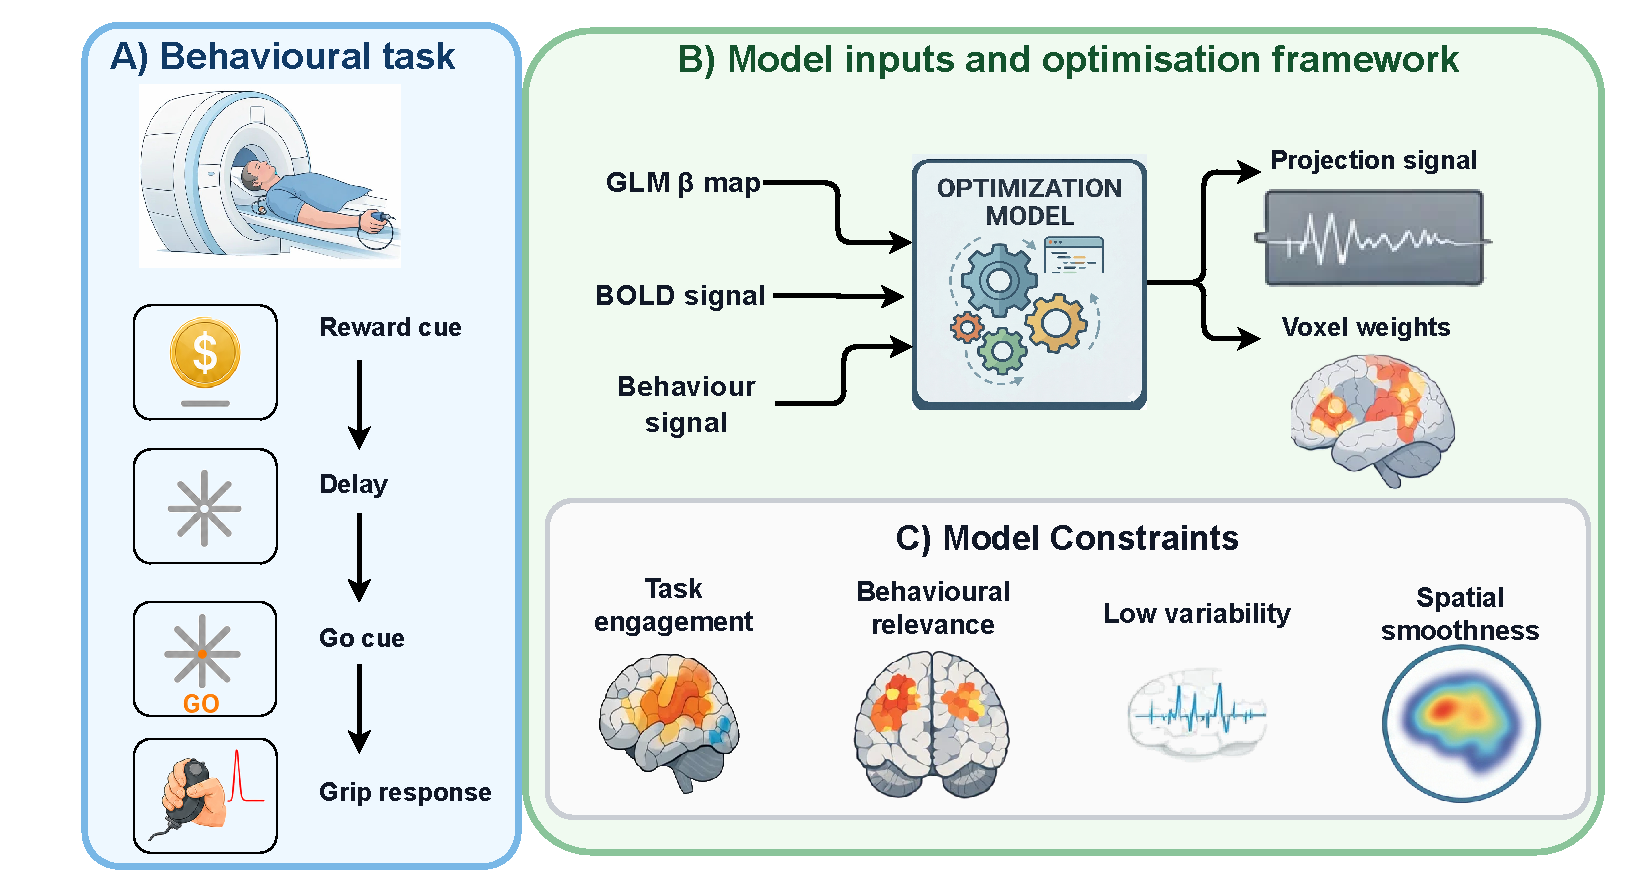
\includegraphics[width=\textwidth]{main_figures/Figure1.pdf}
    \caption{Overview of the behavioural task and analysis pipeline. \textbf{A}, The task panel shows a reward cue, variable delay, Go signal, grip response, and recorded reaction-time and whole-brain BOLD measures. \textbf{B}, The analysis panel shows GLMsingle single-trial beta estimates, BOLD-derived features, reaction-time measures, and the constrained optimisation inputs and outputs. \textbf{C}, The optimisation panel shows the task-engagement, behaviour-association, spatial-coherence, and trial-to-trial stability terms used to estimate the projection signal and voxel-weight map.}
    \label{fig:task_analysis_overview}
\end{figure}

\clearpage
\begin{figure}[!p]
    \centering
    \begin{minipage}{\textwidth}
        \noindent\textbf{A}\par\vspace{0.2em}
        \centering
        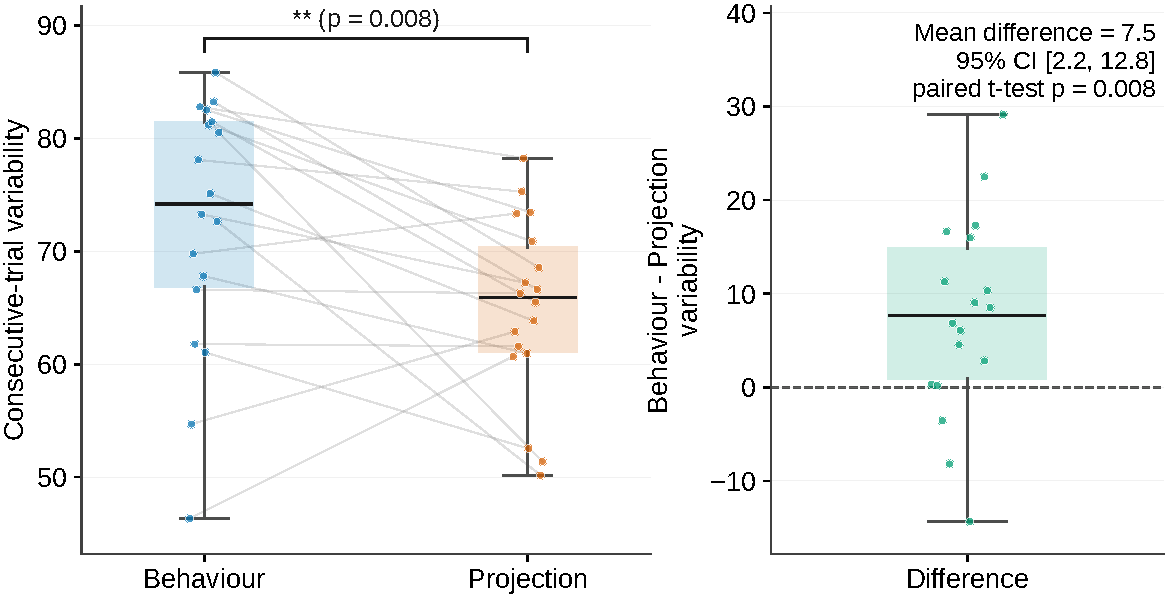
\includegraphics[width=0.88\textwidth]{main_figures/Figure2A.pdf}
    \end{minipage}\par\vspace{0.8em}
    \begin{minipage}{\textwidth}
        \noindent\textbf{B}\par\vspace{0.2em}
        \centering
        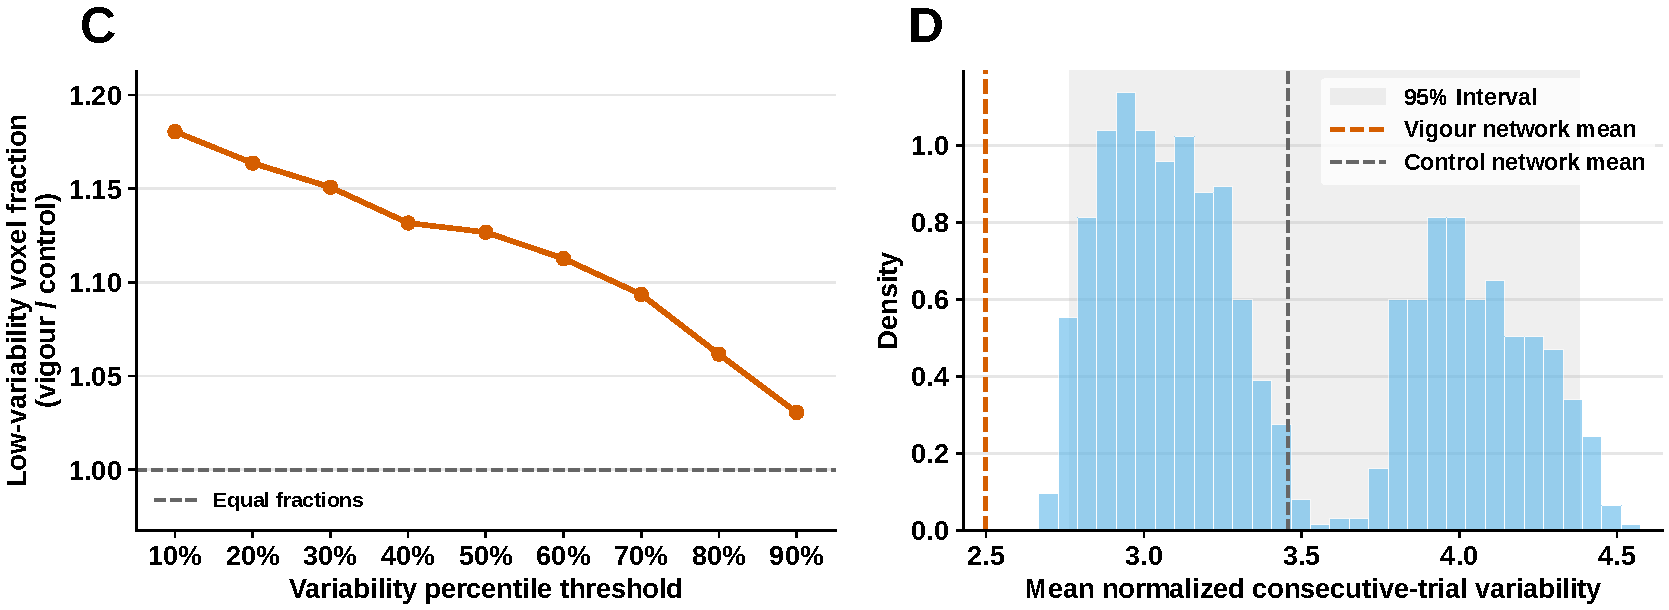
\includegraphics[width=0.98\textwidth]{main_figures/Figure2B.pdf}
    \end{minipage}
    \caption{Validation displays for the optimisation framework. \textbf{A}, The paired plot compares consecutive-trial changes in the optimised neural projection with consecutive-trial changes in reaction time. Positive behaviour-minus-projection values indicate cases where the behaviour change exceeds the projection change. ($n = 18$ subjects, $70$ runs; mean behaviour-minus-projection difference = $7.8, 95\%$ CI $[2.9, 12.7]$; paired $t$-test, $t(17) = 2.98$, $p = 0.004$).\textbf{B}, The voxel-stability panels compare vigour network voxels with size-matched other voxels in motor areas and show the distribution of voxel beta-variability rankings. Selected voxels in the vigour network showed lower mean consecutive-trial beta variability than the size-matched control resamples (selected mean = $2.50$; control-resample mean = $3.46; 95\%$ resampling CI $[2.76, 4.38]$; empirical p $= 0.001$ from $1,000$ resamples). Selected voxels were more prevalent in lower-variability bins, with vigour/control fraction ratios ranging from $1.18$ at the $10th$ percentile to $1.03$ at the $90th$ percentile.}
    \label{fig:optimization_validation}
\end{figure}

\clearpage
\begin{figure}[!p]
    \centering
    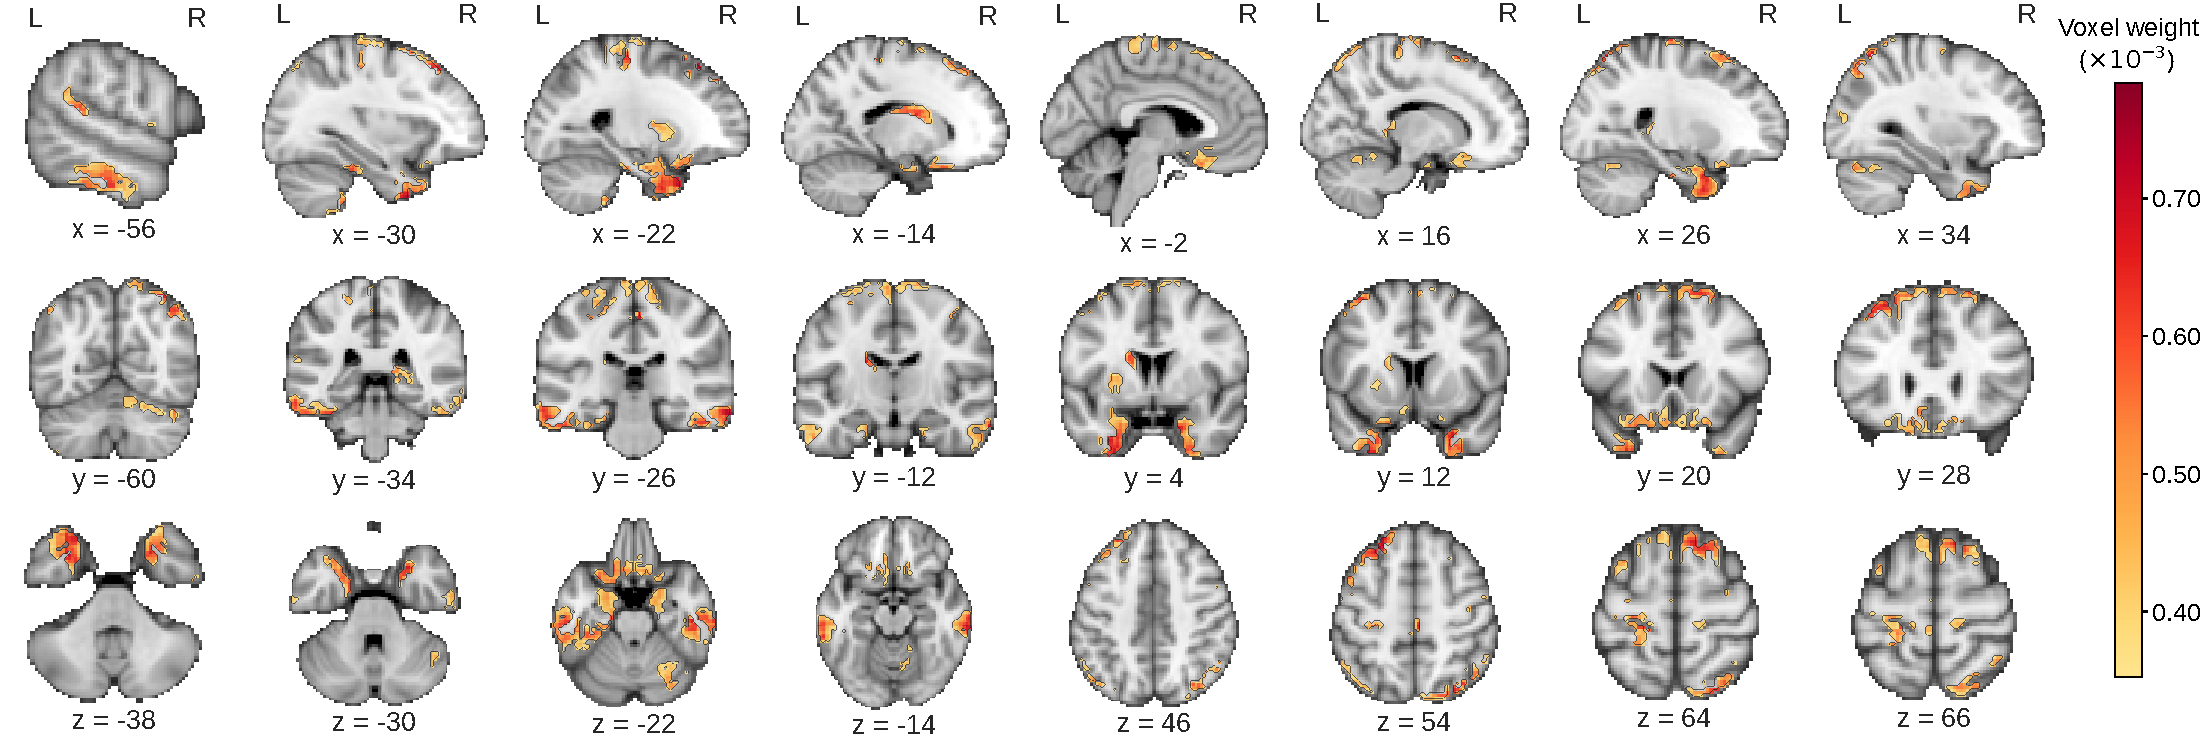
\includegraphics[width=\textwidth]{main_figures/Figure3.pdf}
    \caption{Spatial distribution of the vigour network. Thresholded voxel weights are shown on representative sagittal, coronal, and axial MNI slices. Warmer colours show larger model-derived voxel contributions, scaled by \(10^{-3}\).}
    \label{fig:main_vigour_network}

    \vspace{1.2em}
    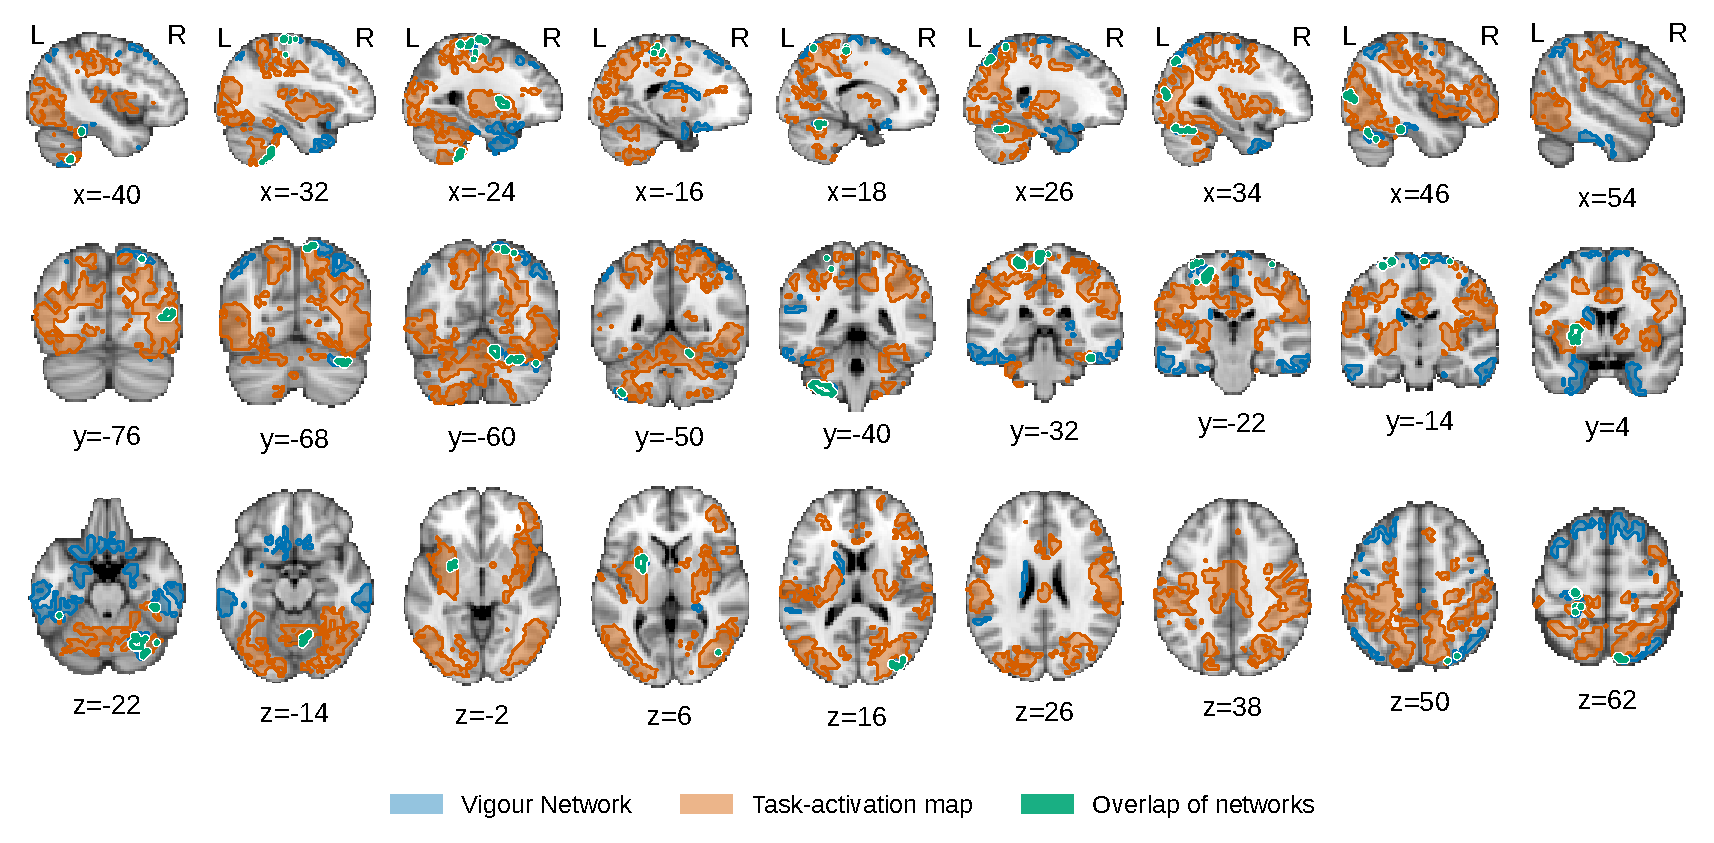
\includegraphics[width=\textwidth]{main_figures/Figure4.pdf}
    \caption{Voxelwise overlap between the vigour network and the standard task-activation map. Blue marks the vigour network, orange marks the task-activation map, and green marks the same-voxel overlap across representative brain slices.}
    \label{fig:main_network_task_overlap}
\end{figure}

\begin{figure}[!htbp]
    \centering
    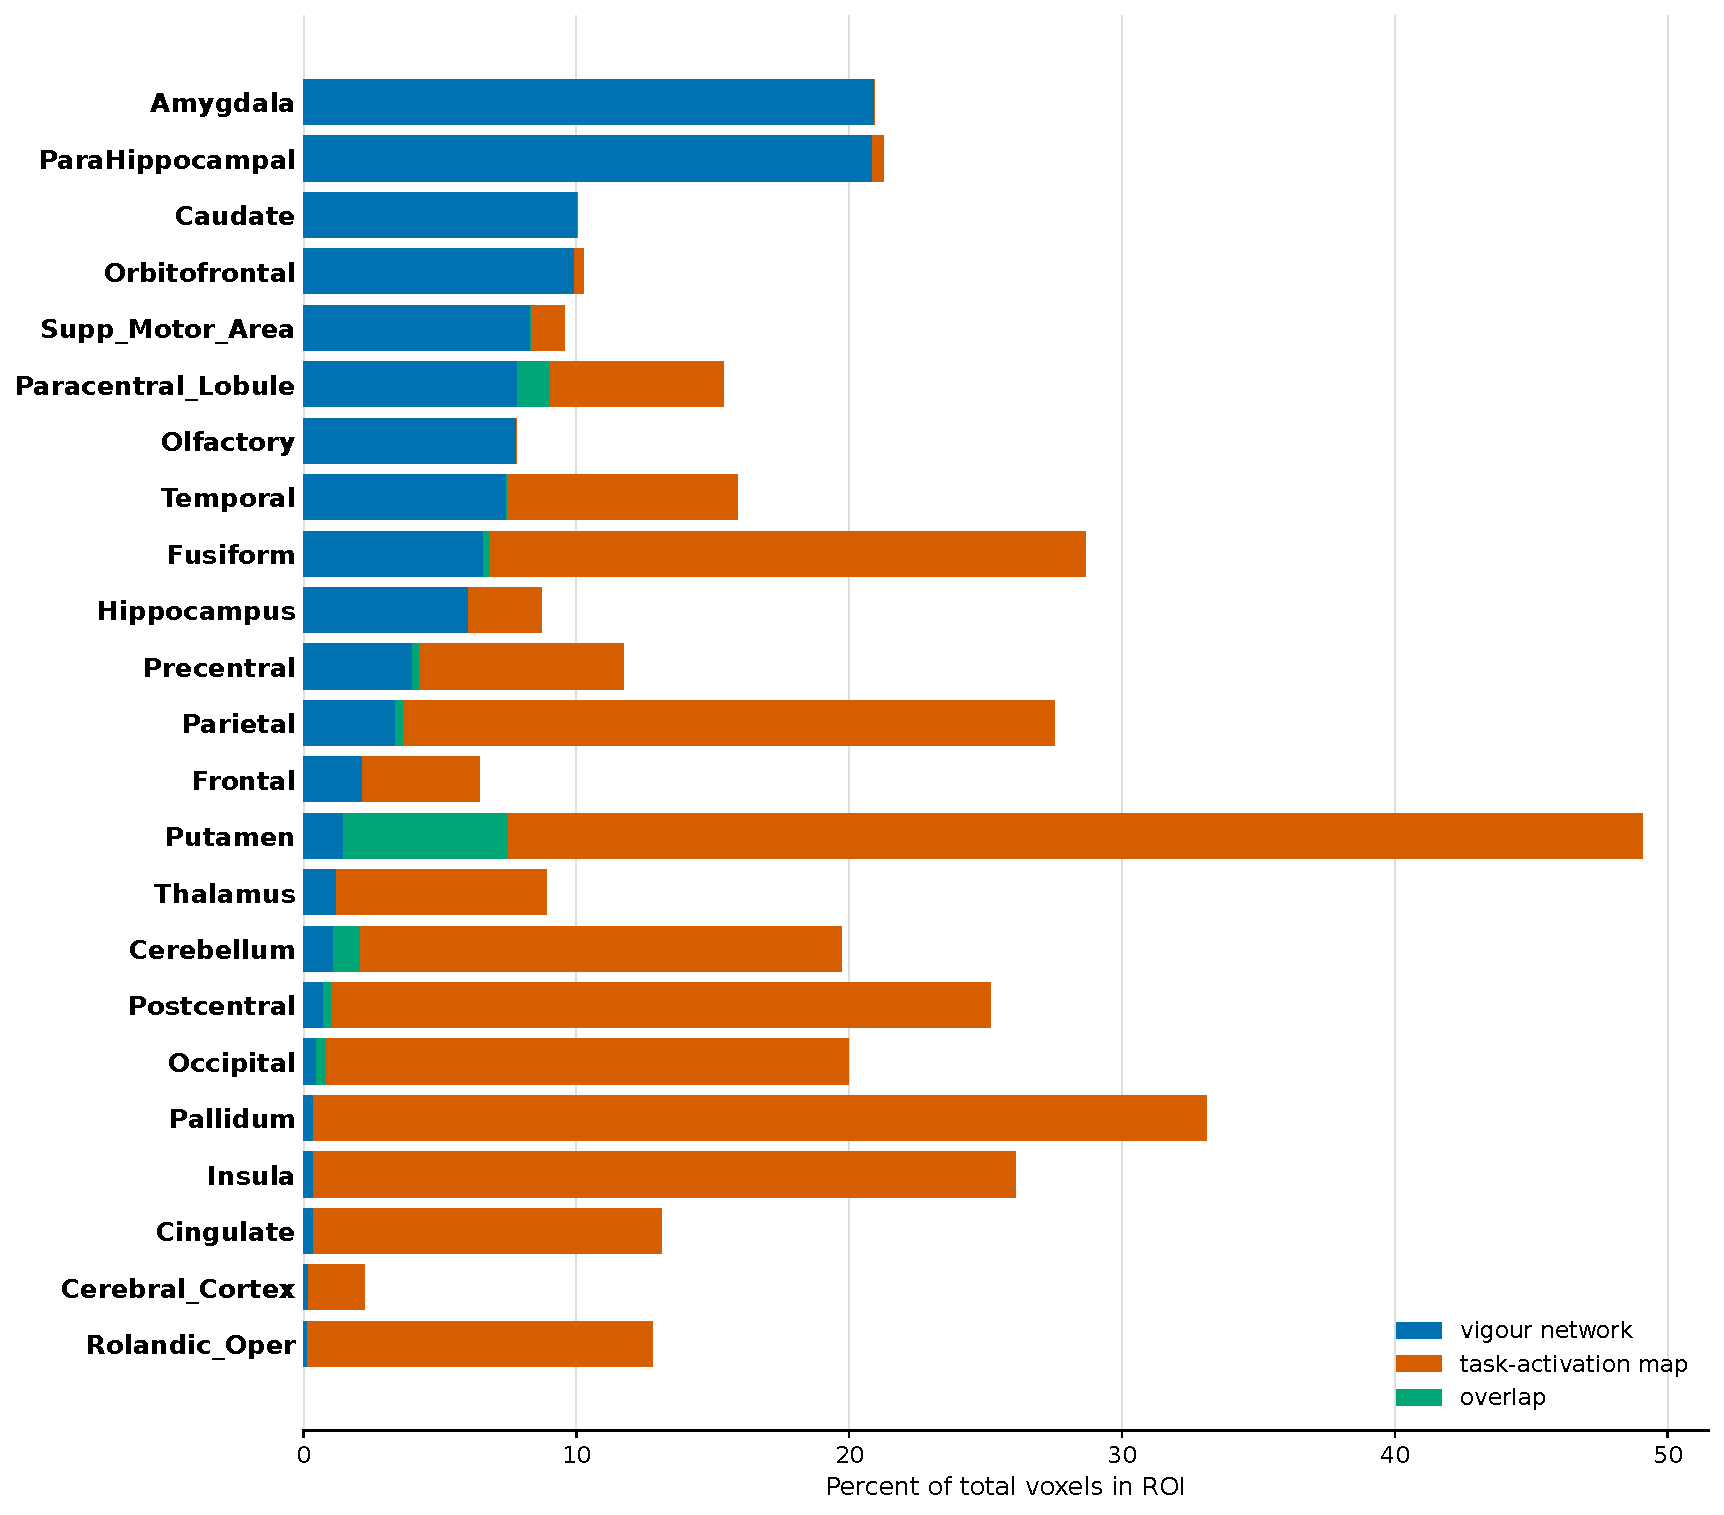
\includegraphics[width=\textwidth]{main_figures/Figure5.pdf}
    \caption{Anatomical comparison by ROI for the vigour network, the standard task-activation map, and their same-voxel overlap. Horizontal bars show the percentage of each ROI occupied by the vigour network, the task-activation map, and overlapping voxels. ROI labels are grouped by anatomical sector, with separate bars for vigour, task activation, and overlap values.}
    \label{fig:roi_task_overlap_summary}
\end{figure}

\begin{figure}[!htbp]
    \centering
    \begin{minipage}{\textwidth}
        \centering
        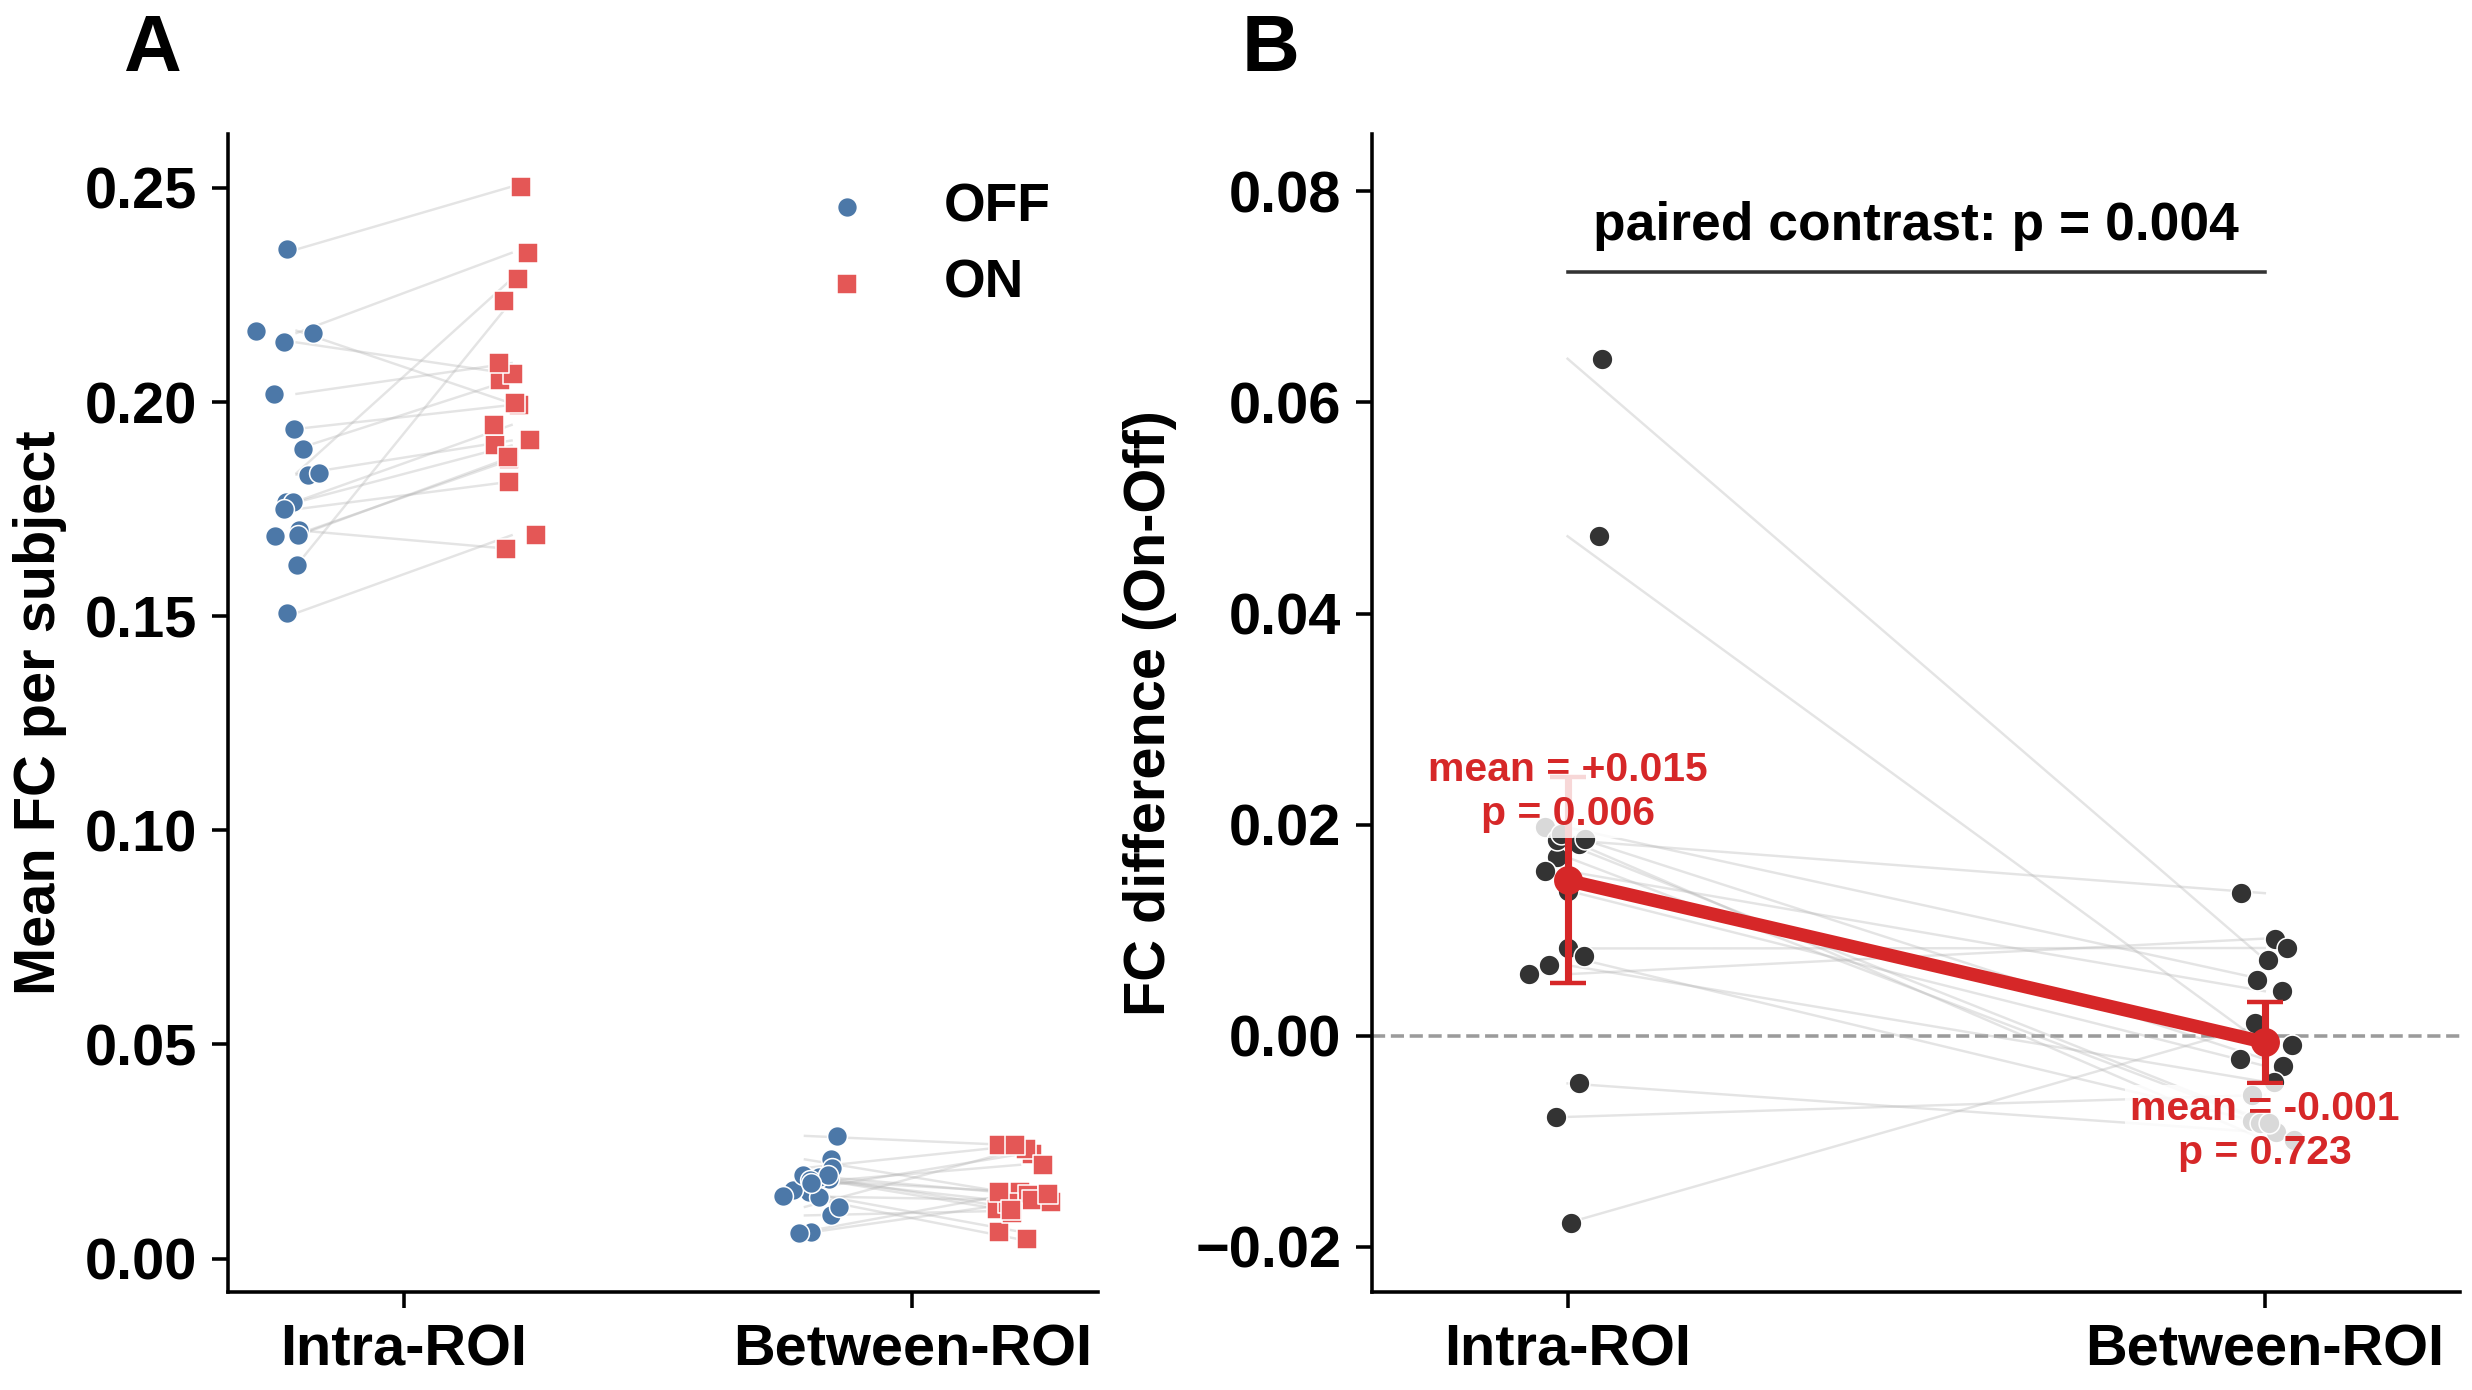
\includegraphics[width=0.92\textwidth]{main_figures/Figure6A.pdf}
    \end{minipage}\par\vspace{0.35em}
    \begin{minipage}{\textwidth}
        \centering
        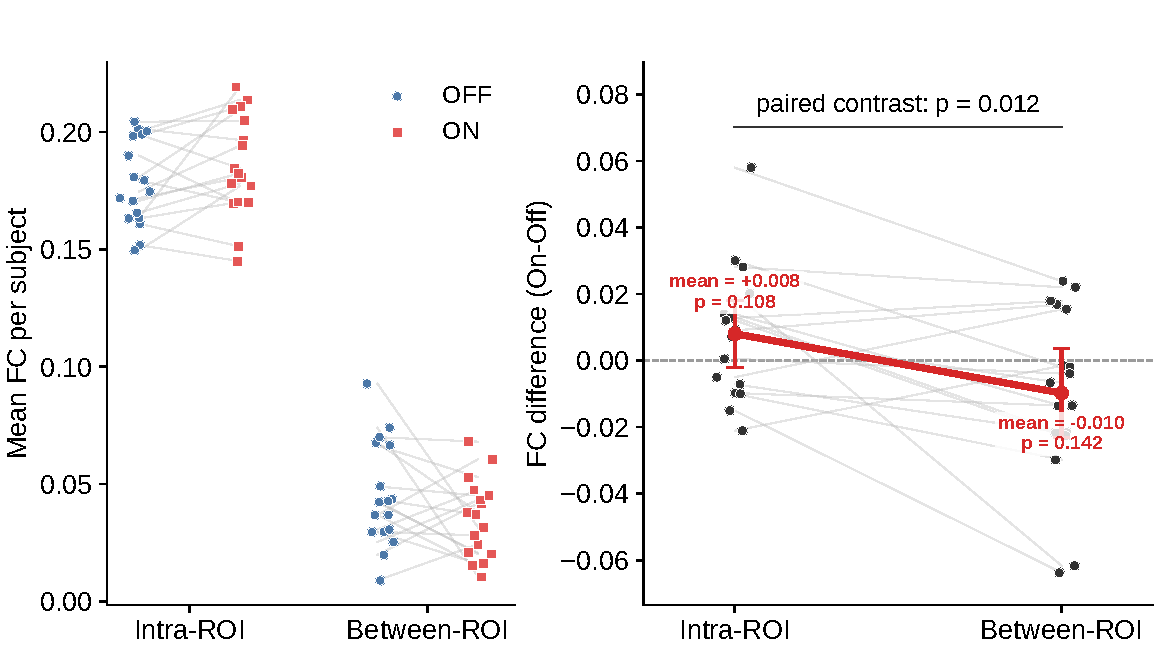
\includegraphics[width=0.92\textwidth]{main_figures/Figure6B.pdf}
    \end{minipage}
    \caption{Medication-state functional connectivity summaries. For the vigour network, plots show within-ROI and between-ROI Pearson functional connectivity for OFF medication, ON medication, and participant-level ON--OFF differences. The corresponding plots show within-ROI and between-ROI Pearson functional connectivity for the standard task-activation map.}
    \label{fig:medication_local_distributed_fc}
\end{figure}

\clearpage
\begin{figure}[!p]
    \centering
    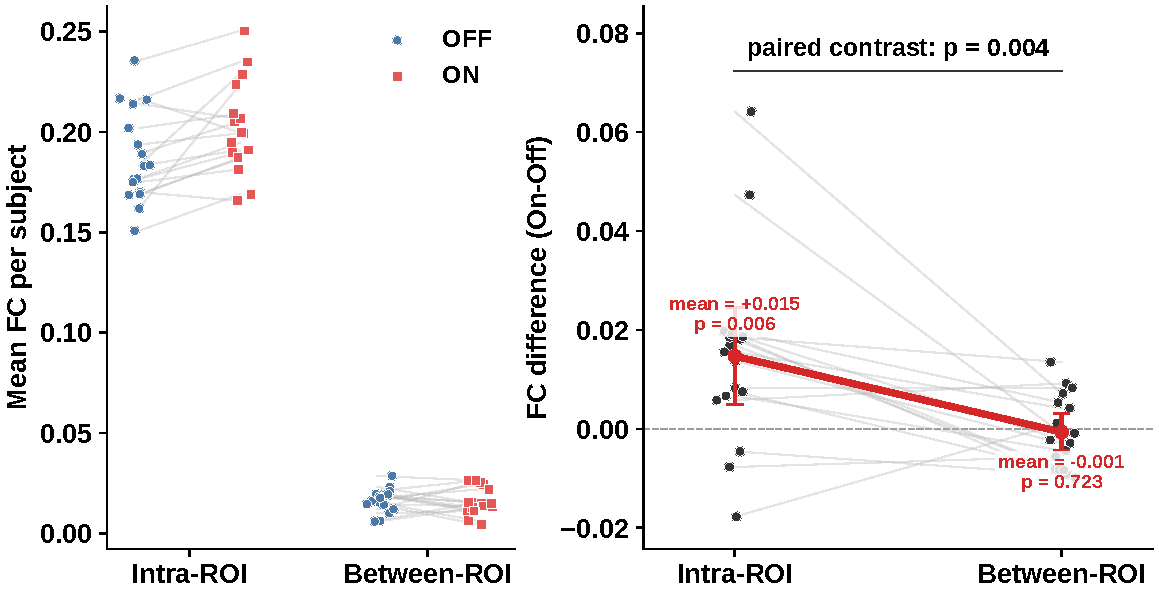
\includegraphics[width=0.96\textwidth]{main_figures/Figure8A.pdf}

    \vspace{0.25em}

    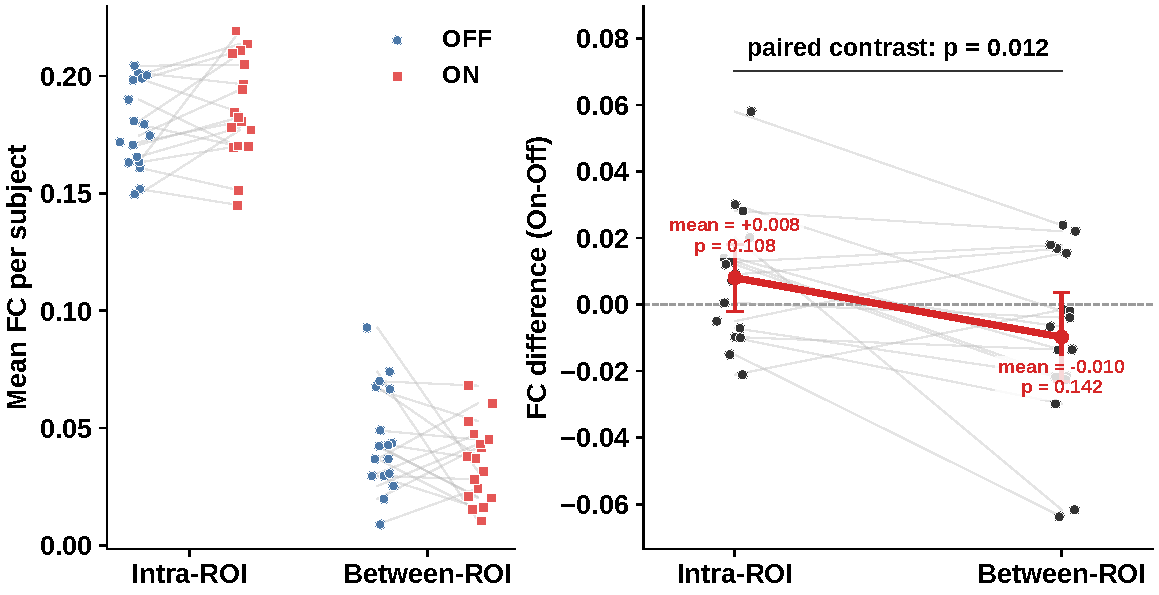
\includegraphics[width=0.96\textwidth]{main_figures/Figure8B.pdf}

    \vspace{0.25em}

    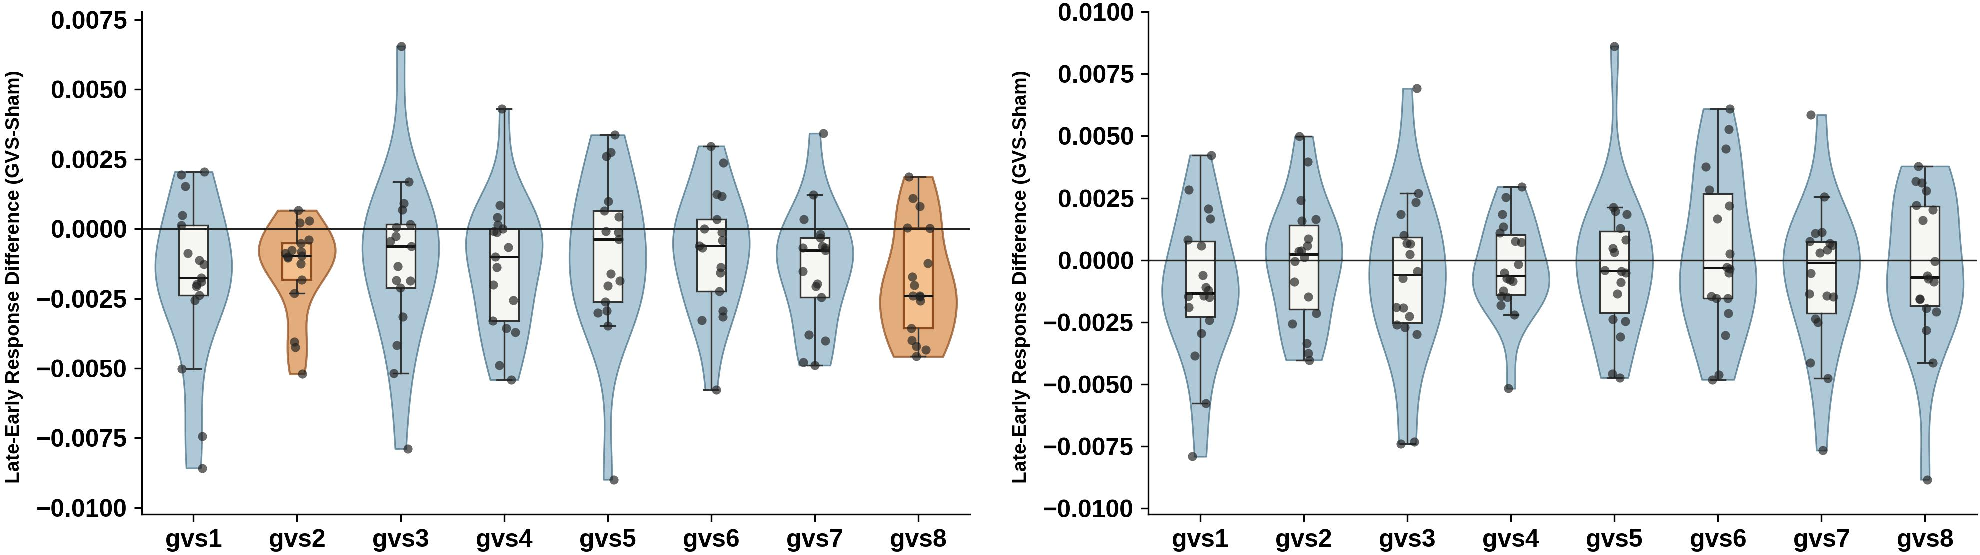
\includegraphics[width=0.96\textwidth]{main_figures/Figure8C.pdf}
    \caption{GVS effects on reaction time and projected signal dynamics. Top row: normalized reaction time across sham and GVS1-GVS8 conditions during medication OFF (A) and medication ON (B); lower normalized RT indicates faster responses, and error bars show SEM. Middle row: subject-level GVS-minus-sham late-minus-early response differences from the vigour network projected signal. Bottom row: the same late-minus-early feature computed from the task-activation map BOLD signal. In the neural panels, violins show the subject distribution, boxes show median/IQR, and points show individual subjects after pairing each active GVS condition with sham within subject/session/run. The horizontal zero line indicates no difference from sham. Orange highlights GVS conditions surviving multiple-comparison correction; blue indicates non-significant active GVS conditions.}
    \label{fig:gvs_behaviour_network_responses}
\end{figure}

\begin{figure}[!p]
    \centering
    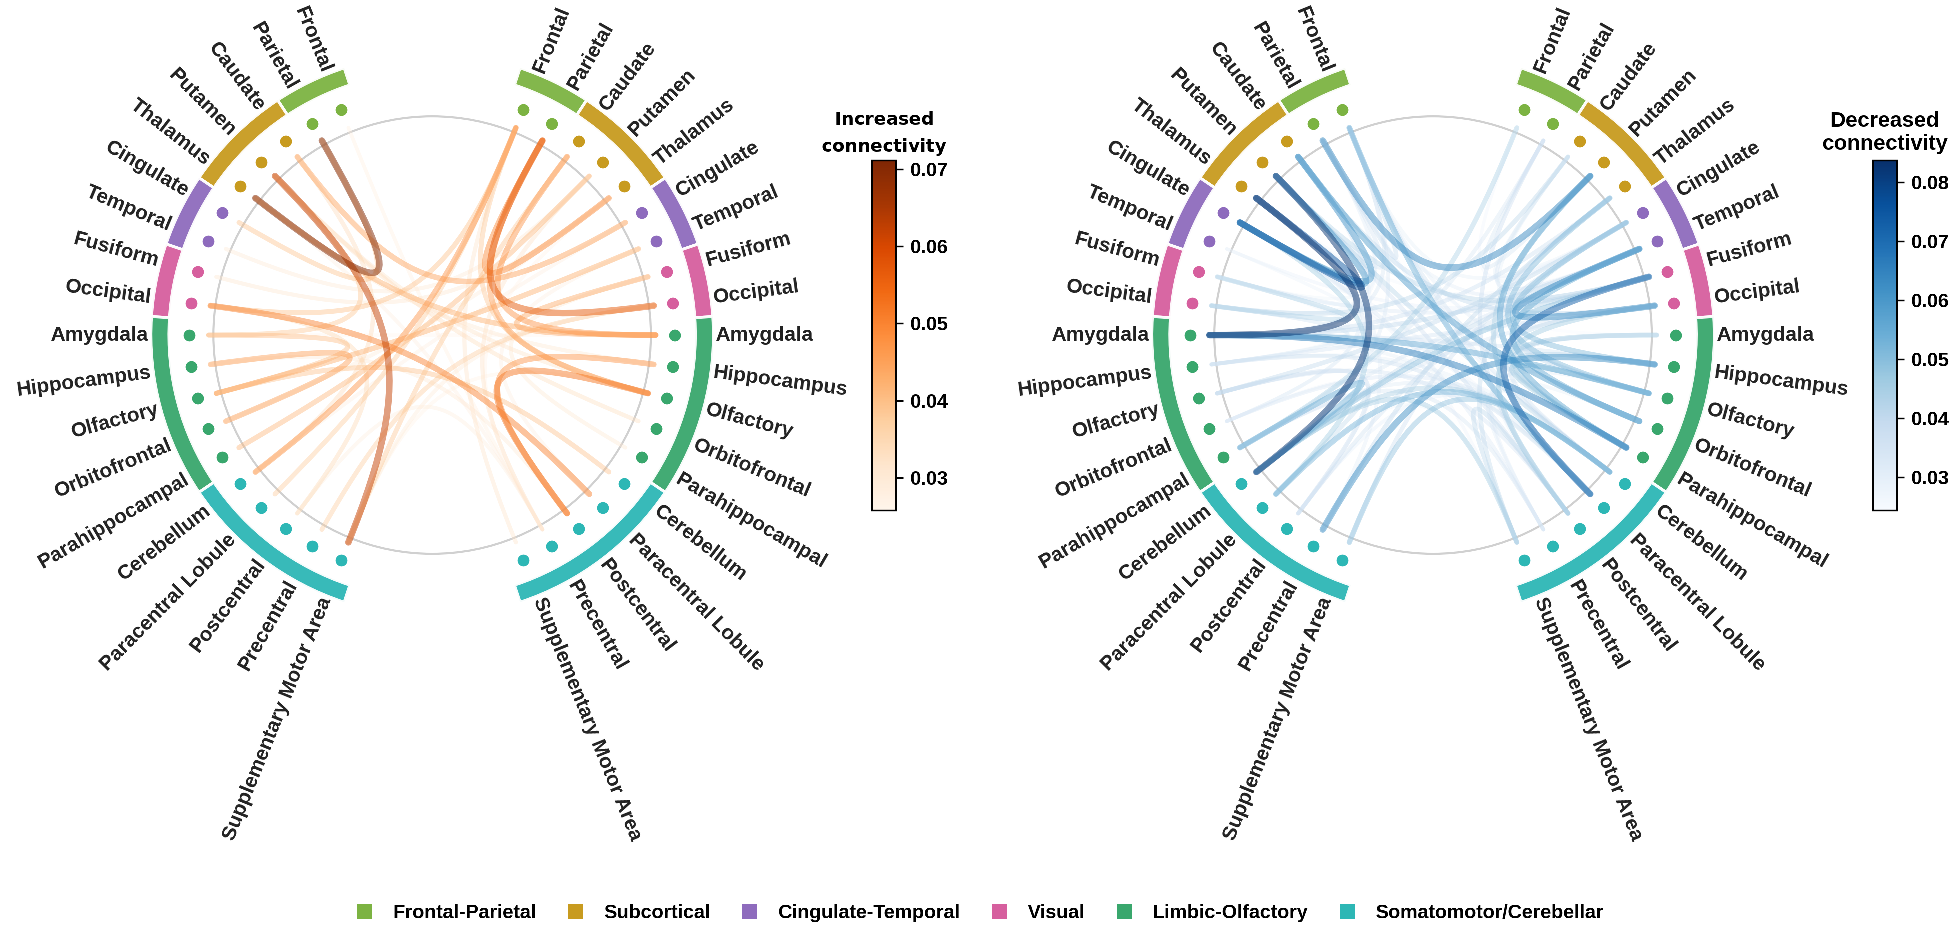
\includegraphics[width=\textwidth]{main_figures/Figure7.pdf}
    \caption{Exploratory GVS-related mutual-information edge changes in the vigour network. Active--sham edge changes that were significant after FDR correction are shown separately for increased and decreased connectivity. Changes were pooled across subjects, medication states, runs, and active GVS waveforms. Orange edges mark increased statistical dependence, and blue edges mark decreased statistical dependence; colour intensity scales with the mean edge-change magnitude. Nodes are labelled by ROI and grouped by anatomical sector.}
    \label{fig:gvs_edge_changes}
\end{figure}



\FloatBarrier
\end{document}
